% Unified CO2Flux report. Compile from Project_description/Research_log
% Source commit: 5fb1ca89260192f189d69ac73fa360caec7598d5
% latexmk -pdf -interaction=nonstopmode -halt-on-error Research_Report.tex
\documentclass[11pt,letterpaper]{article}
\usepackage[T1]{fontenc}
\usepackage[utf8]{inputenc}
\usepackage{lmodern,amsmath,amssymb,graphicx,booktabs,longtable,pdflscape,geometry,hyperref,microtype}
\geometry{margin=0.85in}
\hypersetup{colorlinks=true,linkcolor=blue,urlcolor=blue,pdfauthor={Dimitri Bolt}}
\newcommand{\CO}{\mathrm{CO}_2}
\newcommand{\Arg}{\operatorname{Arg}}
\newcommand{\wrap}{\operatorname{wrap}}
\title{CO2Flux: Relative Spectral Phases of Subsurface CO$_2$ at Biosphere 2 LEO\\
\large A Unified Report of Documented Results and Open Validation}
\author{Dimitri Bolt\\{\small Academic Advisor: Professor Ildar R. Gabitov}}
\date{28.Oct.2026}
\begin{document}
\maketitle
\begin{abstract}
I summarize the documented CO$_2$ analyses at Biosphere 2 LEO
without changing my approved research plan. For vertical
W\_x1\_y4, the accepted observation interval is
01.May.2025--30.Sep.2026 (17 complete months).
The limited Stage 0.1-B hydrological input consists of
14 series and 37 indirect wetting dates, not a verified
irrigation-event calendar. Stage 0.2 is closed using my
monthly median daily-amplitude threshold of 2.5 in
each channel's stored units: 6,123 common two-hour cells
and 489 technically computable 30-day windows.
My older four-channel phase demonstration comprises
492 windows obtained with previous input masks; I have
not recomputed those four-channel phases on the accepted
Stage 0.2 input. A newer Stage 0.5 diagnostic compares
15-minute and two-hour subsurface Fourier phases across
489 matched windows for two adjacent depth pairs.
It separates the additional common-cell restriction
caused by the atmospheric sensor. I report both numerical
sensitivity and limitations without deciding whether
two-hour sampling is adequate. The final Stage 0.5
decision by I.~R.~Gabitov and the conditions for new
Chapter 1 remain open.
\end{abstract}
\tableofcontents

\clearpage
\section*{Research roadmap and source correspondence}
\addcontentsline{toc}{section}{Research roadmap and source correspondence}
\label{sec:roadmap}
The identifiers below follow the existing
\href{https://github.com/DimitriBolt/CO2Flux/blob/main/Project_description/Research_log/README.md}{research README}
and the
\href{https://github.com/DimitriBolt/CO2Flux/blob/main/Project_description/Research_log/PLAN.md}{approved PLAN}.
They identify research stages, not the numbered sections of this report.
In particular, \textbf{0.5/Q1} is a completed diagnostic of one phase change,
\emph{not} completion of Stage 0.5. Existing numbered historical
notebooks concern the previous methodology, not the future spectral chapters.

\begingroup
\footnotesize
\setlength{\tabcolsep}{2.8pt}
\renewcommand{\arraystretch}{1.13}
\begin{longtable}{@{}p{1.28cm}p{4.0cm}p{3.35cm}p{5.05cm}@{}}
\toprule
Stage & Object and status & Report section & Canonical source\\
\midrule
0.1-B & Limited hydrological input accepted; full event log missing
& \hyperref[sec:hydro]{Hydrology}
& \href{https://github.com/DimitriBolt/CO2Flux/blob/main/Project_description/Research_log/details/00_irrigation_audit.md#stage01b-pilot-input}{Hydrological audit}\\
0.2 & Accepted 17-month input and author threshold 2.5; closed with limitations
& \hyperref[sec:data]{Data and QC}
& \href{https://github.com/DimitriBolt/CO2Flux/blob/main/Project_description/Research_log/details/02_data_checks.md}{Data checks}\\
0.3 & Preliminary amplitude spectra; calculated, not a final frequency choice
& \hyperref[sec:gls]{Amplitude spectra}
& \href{https://github.com/DimitriBolt/CO2Flux/blob/main/Project_description/Research_log/00_preliminary_co2_spectra.ipynb}{Spectra notebook}\\
0.4 & Earlier 492-window phase demonstration, not recalculated with 489-window input
& \hyperref[sec:fourier]{Direct Fourier}; \hyperref[sec:phase-results]{phase series}
& \href{https://github.com/DimitriBolt/CO2Flux/blob/main/Project_description/Research_log/00_preliminary_fourier_phases.ipynb}{Phase notebook, sections 1--9}\\
0.5/Q1 & One phase jump analyzed; does not close Stage 0.5
& \hyperref[sec:jump]{Single-jump result}
& \href{https://github.com/DimitriBolt/CO2Flux/blob/main/Project_description/Research_log/00_preliminary_fourier_phases.ipynb#one-phase-jump}{Phase notebook, section 10}\\
0.5/grid & 15-minute versus two-hour phases for two subsurface pairs; diagnostic completed
& \hyperref[sec:gridstudy]{Grid comparison}
& \href{https://github.com/DimitriBolt/CO2Flux/blob/main/Project_description/Research_log/00_preliminary_fourier_phases.ipynb#temporal-grid-resolution}{Phase notebook, section 11}\\
0.5 & Presentation to I.G. and explicit approval; pending
& \hyperref[sec:next]{Next approved steps}
& \href{https://github.com/DimitriBolt/CO2Flux/blob/main/Project_description/Research_log/PLAN.md#preparation}{PLAN: 0.5 and stopping criteria}\\
1--3 & Future spectral-phase chapters; not yet begun
& \hyperref[sec:next]{Next approved steps}
& \href{https://github.com/DimitriBolt/CO2Flux/blob/main/Project_description/Research_log/PLAN.md#later}{PLAN: later stages}\\
4 & Buchstaber method; methodological preparation only
& \hyperref[sec:buchstaber]{Buchstaber}
& \href{https://github.com/DimitriBolt/CO2Flux/blob/main/Project_description/Research_log/04_buchstaber.ipynb}{Buchstaber notebook}\\
5--6 & Spatial links and physical mechanisms; future work
& \hyperref[sec:next]{Next approved steps}
& \href{https://github.com/DimitriBolt/CO2Flux/blob/main/Project_description/Research_log/PLAN.md#later}{PLAN: later stages}\\
Historic 1--3 & Absolute-harmonic maximum times/amplitudes; distinct earlier work
& \hyperref[sec:historical]{Historical analyses}
& \href{https://github.com/DimitriBolt/CO2Flux/blob/main/Project_description/Research_log/01_october_2017.ipynb}{Notebook 01},
\href{https://github.com/DimitriBolt/CO2Flux/blob/main/Project_description/Research_log/02_monthly_changes.ipynb}{02},
\href{https://github.com/DimitriBolt/CO2Flux/blob/main/Project_description/Research_log/03_long_term_evolution.ipynb}{03}\\
\bottomrule
\end{longtable}
\endgroup
\clearpage
\newpage
\section{Introduction and research status}
\label{sec:intro}
The long-term objective is to assess whether changes in CO$_2$ accompanying the transformation of crushed basalt into soil allow transport, chemical interactions and biological sources or sinks to be distinguished. The immediate approved observable is instead precisely defined: three relative spectral phases between consecutive levels. Absolute times of fitted diurnal maxima are not interchangeable with these quantities. The current canonical README and PLAN place the project at preparatory Stage 0, before the new Chapter 1 \cite{readme,plan}. This report assembles existing results, not new scientific computations or an alternative research plan.

\section{LEO experimental setup}
\label{sec:setup}
The selected pilot vertical on LEO West is at $(x,y)=(1,4)$ m. Four channels are used: air, 5, 20 and 50 cm. The air LI-COR instrument is at $(0,4)$ m, horizontally 1 m from the basalt profile. Its nominal height $+0.25$ m comes from Excel metadata and is not independently established by the Oracle BOXZ field. The assumption $C_0(t)=C_{\rm air}(t)$ is adopted for the present analysis and must not be mistaken for experimental proof of an exact surface boundary condition \cite{phase,passport}.
\begin{center}
\begin{tabular}{llll}
\toprule
Level & Sensor & Model & Stored unit\\
\midrule
Air & 1275 & LI-COR & $\mu$mol/mol\\
5 cm & 996 & GMM222 & ppm\\
20 cm & 1012 & GMM222 & ppm\\
50 cm & 1035 & GMM222 & ppm\\
\bottomrule
\end{tabular}
\end{center}
The historical West-slope profile W\_R4\_C-4 is different: sensors 994/1010/1026 at 5/20/35 cm. Its results are not pooled with this four-channel 5/20/50 cm pilot.

\section{Hydrological context: accepted Stage 0.1-B input}
\label{sec:hydro}
For the interval 01.May.2025--30.Sep.2026 I accepted
14 hydrological time series: two 5TM volumetric-water-content
(VWC) channels, two MPS-2 matric-potential channels, and ten
separate Model3130 stored-mass channels. The existing source
export contains 696,136 rows, including 289 service values
of $-9999$. The original time stamps, sensor identifiers,
real gaps, service values, and monthly coverage are preserved;
no missing concentrations or hydrological measurements were
interpolated \cite{hydroaudit,hydrovalidation}.

VWC sensors 19/317 (\%) are at neighboring coordinate $(2,4)$,
depths 5 and 35~cm, approximately one meter from my CO$_2$
vertical. MPS-2 sensors 668/889 (kPa) are at W\_x1\_y4,
depths 20 and 50~cm. The ten stored masses 1066--1075 (kg)
refer to support locations across the slope, and I do not
equate them with the amount of supplied water or the water
content of the selected CO$_2$ profile. No conversion from
matric potential to VWC is made without an appropriate
water-retention relationship.

I retained \textbf{37 calendar dates of independently
corroborated wetting}. These are indirect observations,
not 37 verified operational irrigation events.
A complete SCADA log specifying start/end times,
zone, water volume and flow has not been recovered.
Thus Stage 0.1-B is complete for the authorized pilot,
while the original full-event-calendar question remains open.

\begin{figure}[htbp]
\centering
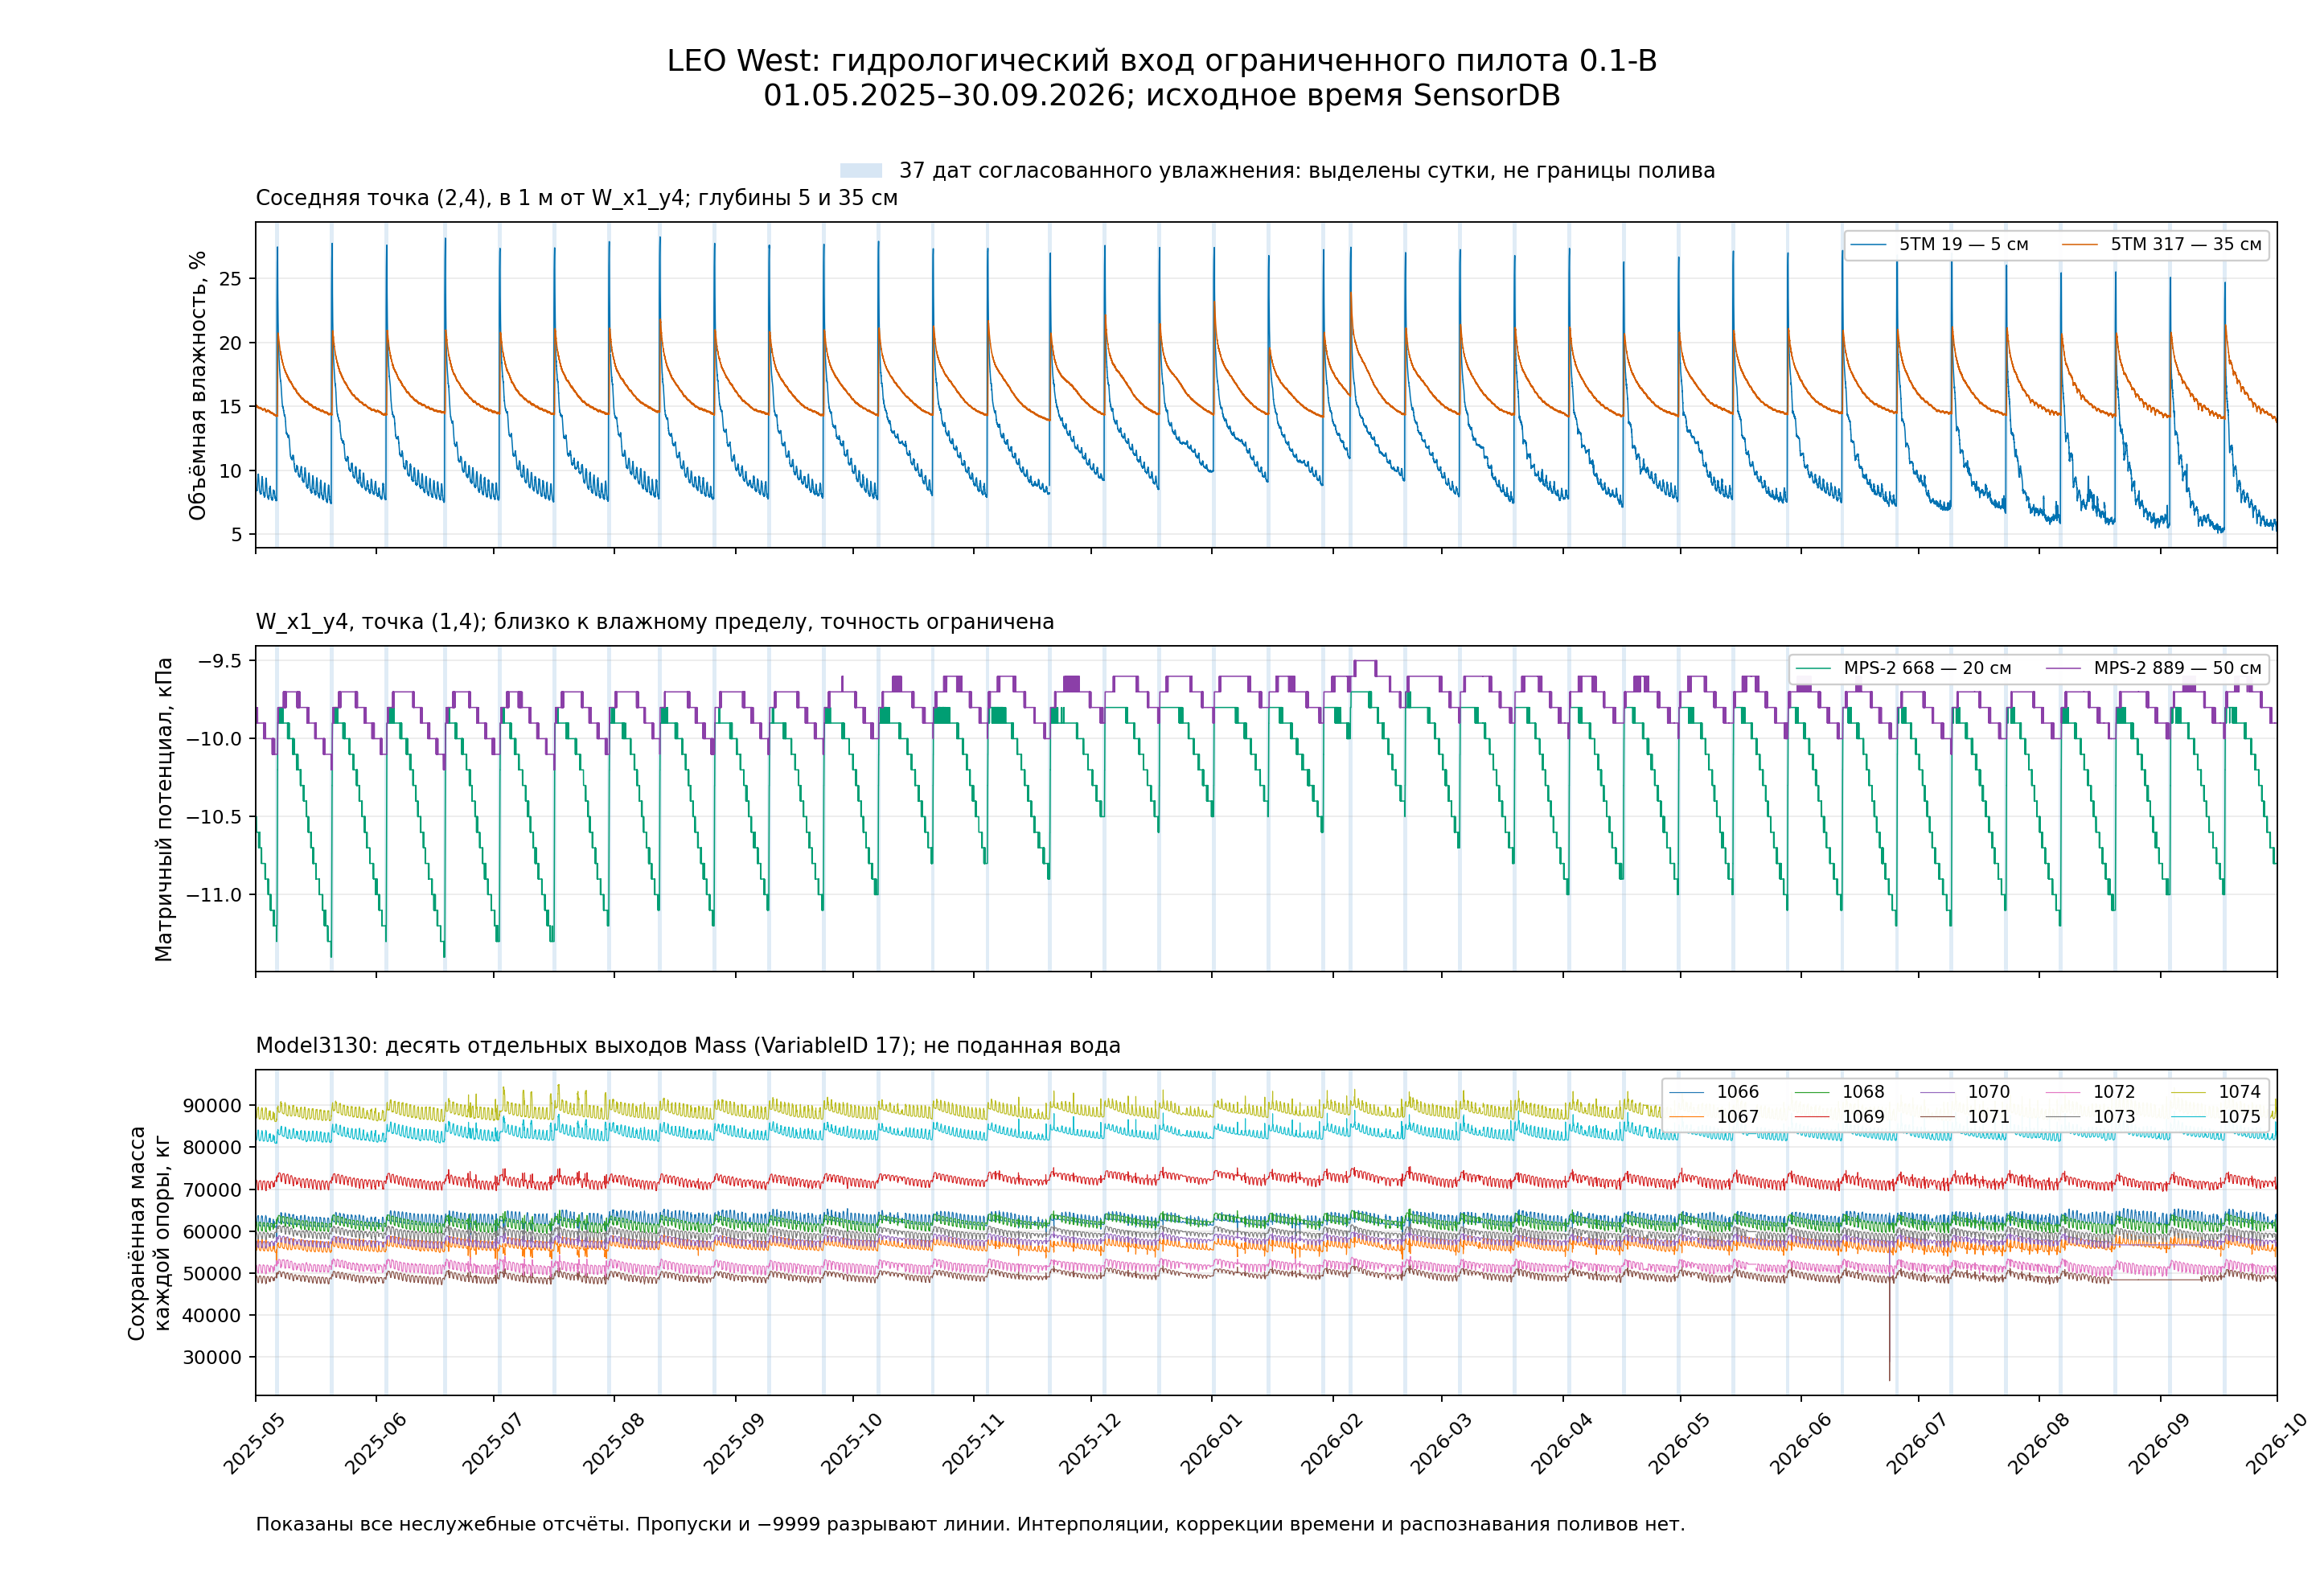
\includegraphics[width=.96\linewidth]{output/stage01_irrigation/pilot_hydrology_17months.png}
\caption{Existing 17-month hydrological overview:
neighboring VWC, on-vertical matric potential and
ten separate slope-support masses. The 37 marked days
identify wetting evidence, not exact irrigation events.}
\label{fig:hydrology}
\end{figure}

\section{Data and quality control}
\label{sec:data}
\subsection{Accepted vertical and scientific scope of Stage 0.2}
I selected W\_x1\_y4 with LI-COR 1275 (air) and GMM222
996/1012/1035 (5, 20, 50~cm). After checking all 16
candidate West-slope verticals, I closed Stage 0.2 on
23.Oct.2026 with the half-open interval
$[01.\mathrm{May}.2025,01.\mathrm{Oct}.2026)$:
\textbf{17 consecutive complete months} with
actual data gaps retained \cite{stage02,stage02validation}.

I approved a minimum monthly median diurnal amplitude
of \textbf{2.5} in each channel's original units:
ppm for GMM222 and $\mu$mol/mol for LI-COR.
This was my separate decision and does \emph{not}
replace or claim to be I.~R.~Gabitov's original
8-unit threshold. The strict-passport result at 8
remains unchanged. My accepted Fourier input selector
is \texttt{technically\_retained \& \textasciitilde doubtful};
it preserves the original observations and rejection
reasons elsewhere. The accepted database time reference
is not shifted.

On this view I obtained \textbf{517 of 518 common days}
and \textbf{6,123 of 6,216} possible two-hour common
cells (98.50\%). The removal of doubtful values lost
25 previously occupied common cells.
The accepted 30-day / one-day-step calendar has
\textbf{489 technically computable windows}, each
with 316--360 common two-hour cells.
This is a data-availability result: it does not mean
489 independently corroborated four-channel phase
calculations. I have not introduced new $R^2$,
coverage, or Fourier-modulus thresholds.

\subsection{Common cells and preserved missingness}
For a channel $j$ and calendar cell
$B_k=[s_k,s_k+2\,\mathrm{h})$, let $R_{jk}$
be its actually accepted source measurements.
I define
\begin{equation}
n_{jk}=|R_{jk}|,\qquad
x_{jk}=\frac1{n_{jk}}\sum_{r\in R_{jk}}C_{jr}
\quad(n_{jk}>0).
\label{eq:bin}
\end{equation}
For window $W$ I use only shared occupied cells
\begin{equation}
I_W=\{k:B_k\subset W,\ n_{jk}>0\
\text{for all }j=0,1,2,3\},\qquad N=|I_W|.
\label{eq:common}
\end{equation}
No absent cell is replaced by zero, no interpolation
or unlimited atmospheric forward-fill is performed,
and the actual calendar is not compressed. The
15-minute comparison below uses separate common
cells of the three subsurface channels.

\subsection{Older pilot results remain distinguished}
The surviving Stage~0.3 spectra and original
Stage~0.4 figures use an earlier calendar beginning
29.Apr.2025 and older technical masks. That pilot
had 6,184 occupied common two-hour cells out of
6,252 possible and computed 492 windows.
The accepted Stage~0.2 view instead has
6,123/6,216 cells and 489 potential windows.
I retain those historical preliminary plots
\emph{without claiming a recalculation of four-channel
Fourier phases or amplitude spectra using the newly
accepted Stage~0.2 masks} \cite{spectra,passport,validation,stage02}.

\section{Fourier methodology}
\subsection{Stage 0.3: amplitude spectra}
\label{sec:gls}
My previously saved preliminary spectra use a floating-intercept, equal-weight generalized Lomb--Scargle sinusoidal least-squares model at each candidate frequency:
\begin{equation}
C_j(t)\simeq c_j(f)+a_j(f)\cos(2\pi ft)+b_j(f)\sin(2\pi ft)
=c_j(f)+\operatorname{Re}\{Z_j(f)e^{2\pi i ft}\},
\quad Z_j=a_j-i b_j,\quad A_j(f)=|Z_j|.
\label{eq:gls}
\end{equation}
$A_j$ is a fitted sinusoidal semi-amplitude in the source unit, not spectral power. This is not the direct Fourier estimator employed in Stage 0.4. The existing method is implemented by \texttt{gls(t,y,frequency)} and \texttt{grid(days)} in \texttt{Project\_description/sensorDB/preliminary\_spectra.py}. The frequency step is $1/T\simeq0.001921153$ cycles/day for an observed span $T\simeq520.5208$ days, over $0<f<6$ cycles/day. The display bound is not a strict Nyquist claim for irregular sampling. Other spectral peaks are documented, but their mechanisms and an optimal physical frequency have not been established. The 24-hour harmonic remains my provisional demonstration frequency \cite{spectra,qc}.
\begin{landscape}
\begin{figure}[p]
\centering
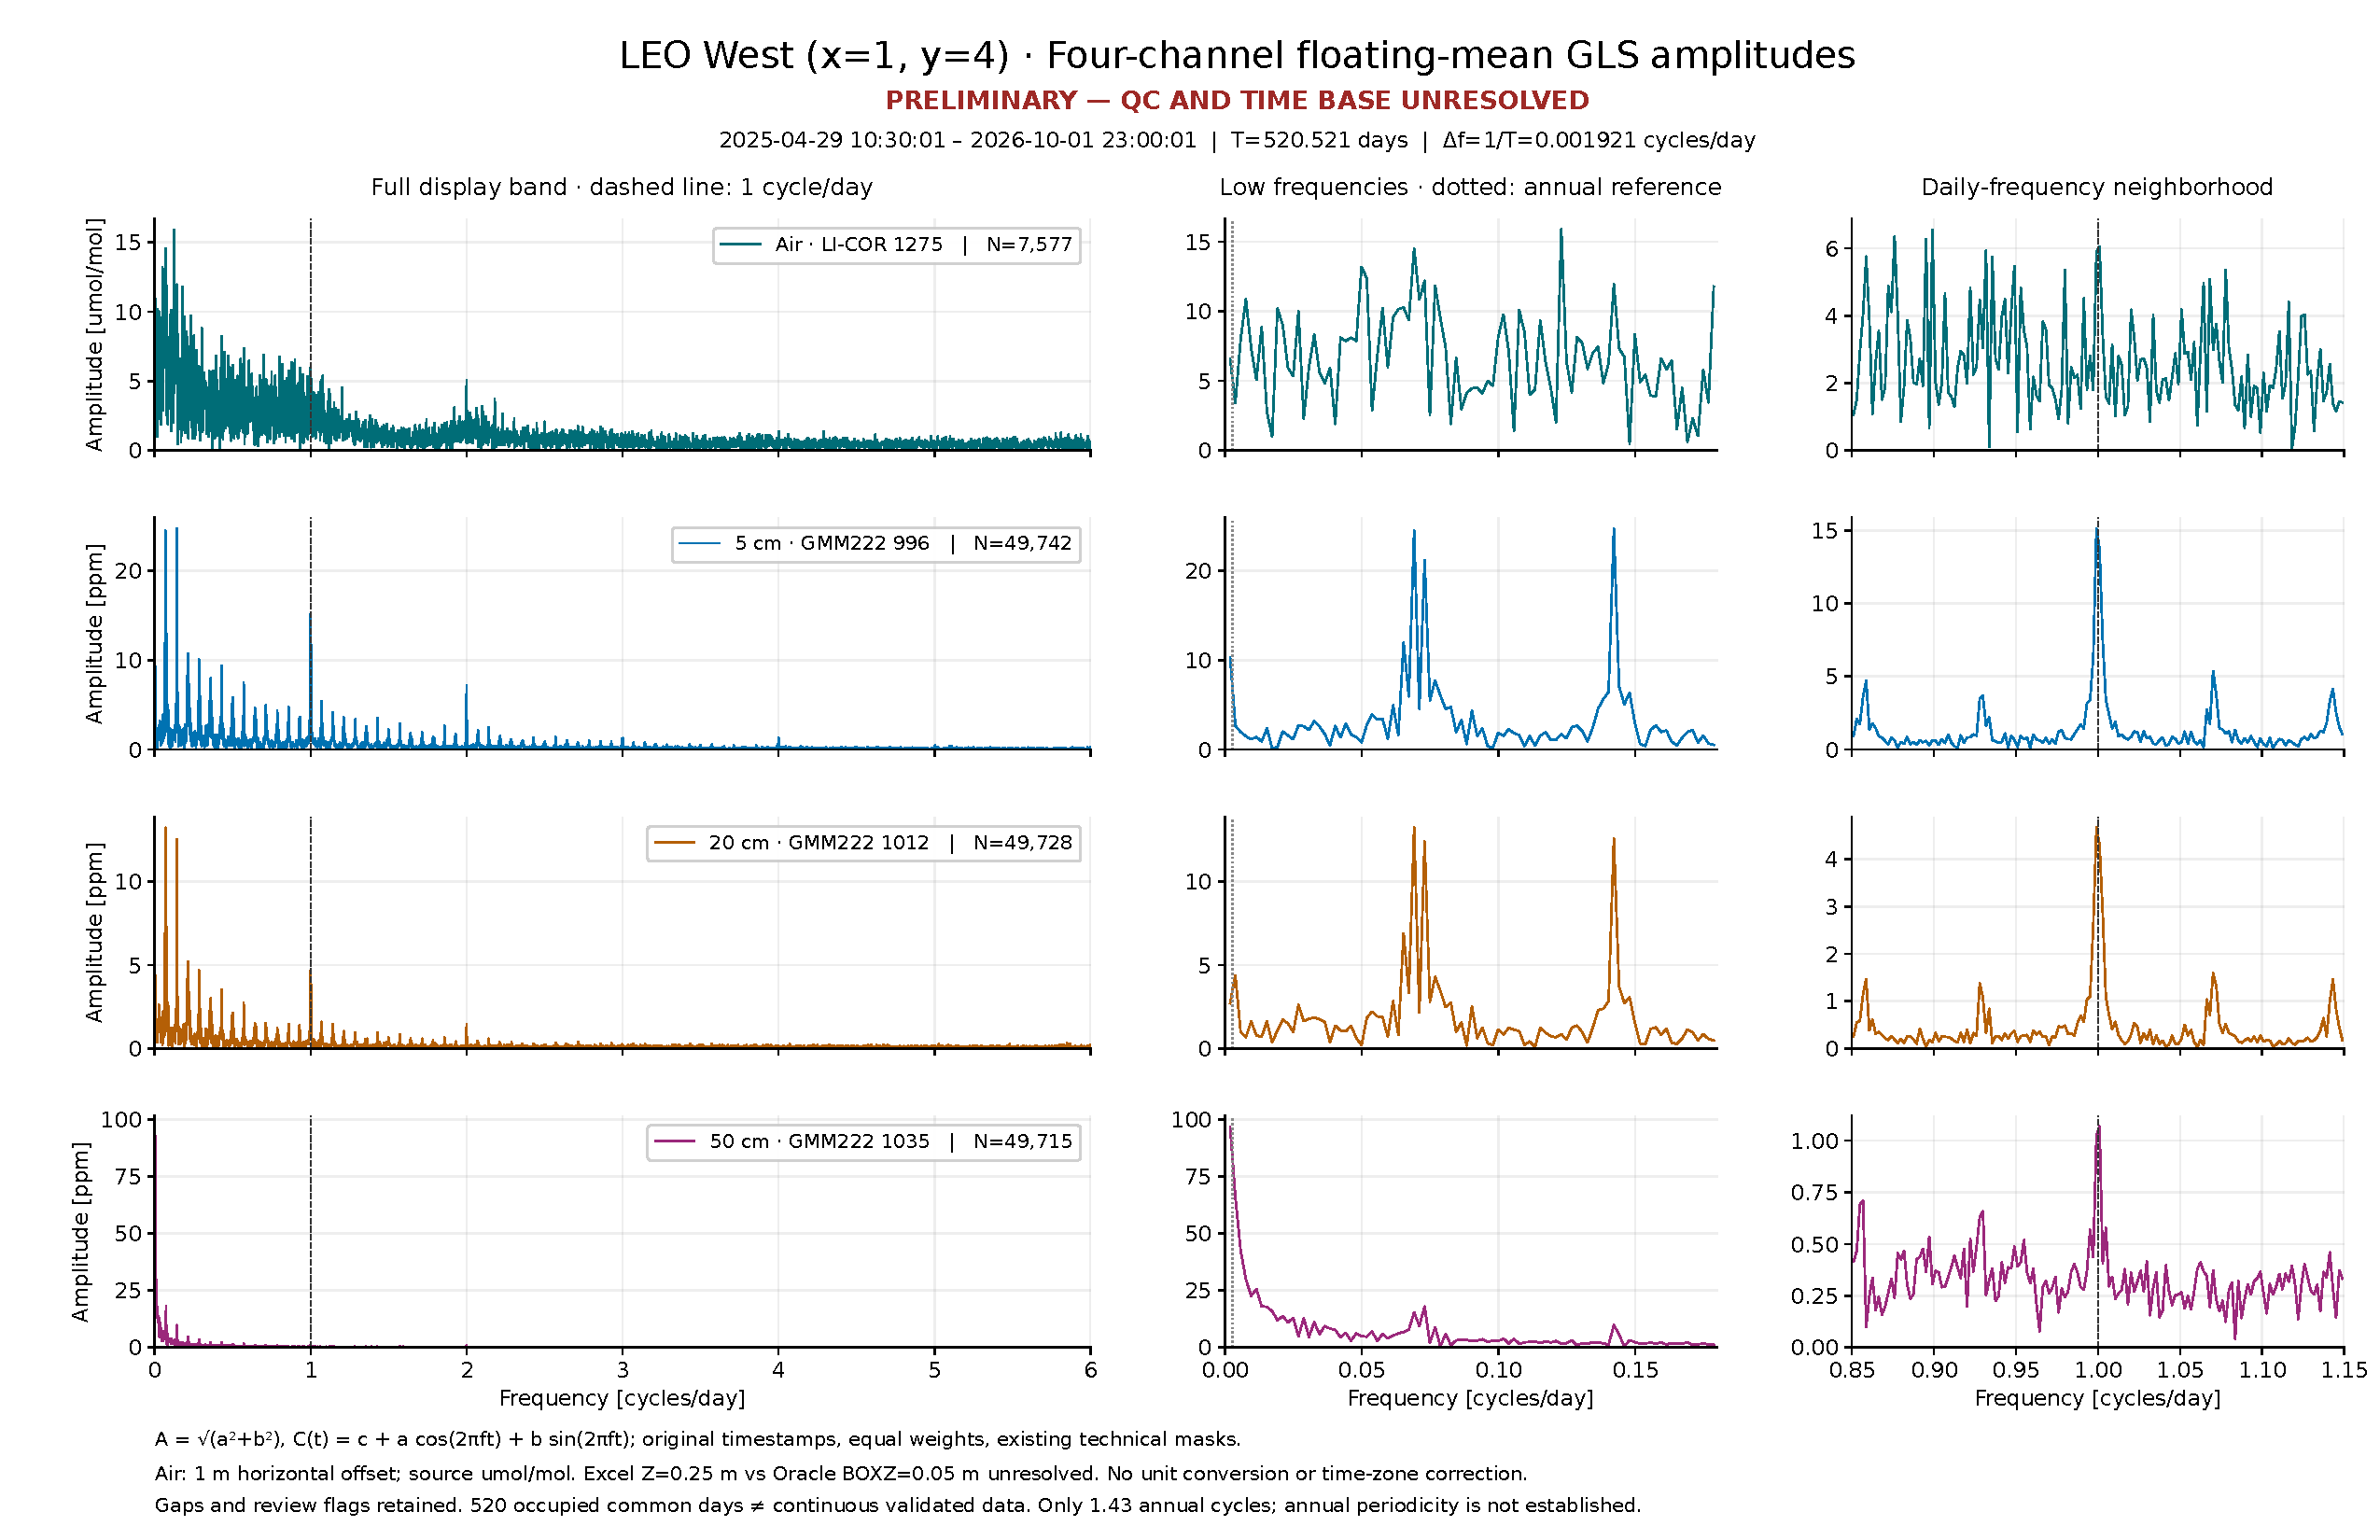
\includegraphics[width=.96\linewidth]{output/preliminary_spectra/four_channel_spectra_17x11.pdf}
\caption{Pre-existing four-channel preliminary amplitude spectra, obtained by independent floating-mean sinusoidal fits. A daily-frequency marker does not constitute frequency selection or phase validation.}
\label{fig:spectra}
\end{figure}
\end{landscape}

\subsection{Stage 0.4: direct complex coefficients and relative phases}
\label{sec:fourier}
For the older Stage~0.4 demonstration I set $t_{\rm ref}=$29.Apr.2025 00:00. For each common two-hour center $t_k=s_k+1$ hour, express $t_k-t_{\rm ref}$ in days. The working frequency is $f_0=1$ cycle/day, window length 30 days, and step one day. For channel $j$ use
\begin{align}
\bar x_{j,W}&=\frac1N\sum_{k\in I_W}x_{jk},\\
F_j(f_0;W)&=\frac1N\sum_{k\in I_W}(x_{jk}-\bar x_{j,W})\,e^{-2\pi i f_0 t_k}.
\label{eq:fourier}
\end{align}
Here $t_k$ is understood relative to the common time origin. Each occupied two-hour cell receives equal weight regardless of its raw observation count. No additional detrending or taper is applied. This is a direct complex Fourier sum on the actual common timestamps, not a gap-compressed FFT or a GLS fit.
For ordered neighboring levels $u\to v$ define
\begin{align}
Q_{uv}&=F_u\overline{F_v},&
\Delta\phi_{u\to v}&=\wrap(\operatorname{Arg}Q_{uv}),\\
\wrap(\alpha)&=(\alpha+\pi)\bmod(2\pi)-\pi\in[-\pi,\pi).
\label{eq:phase}
\end{align}
Thus $\Delta\phi_{\rm air\to5}$, $\Delta\phi_{5\to20}$ and $\Delta\phi_{20\to50}$ are the report's three principal observables. For ideal sinusoidal pairs $u(t)=\cos(\omega_0t)$ and $v(t)=\cos(\omega_0(t-\tau))$ on a complete balanced grid, where $\omega_0=2\pi f_0$, one has $F_u\propto1$ and $F_v\propto e^{-i\omega_0\tau}$; hence
\begin{equation}
\Delta\phi_{u\to v}=\wrap(\omega_0\tau).
\end{equation}
A positive phase denotes a lag of the second \emph{ideal sinusoid}, modulo 24 hours. This identity does not establish a gas-transport lag or transport direction in LEO.

\subsection{Computational implementation and validation}
The existing \texttt{Project\_description/sensorDB/preliminary\_fourier\_phases.py} defines \texttt{aggregate\_bins(frames,start=START,end=END)}, \texttt{direct\_fourier(t\_days,x,f0=F0)}, \texttt{phase\_difference(f\_upper,f\_lower)}, \texttt{wrap(phi)} and \texttt{compute\_windows(grid,window\_days=30,step\_days=1)}. The actual implementation uses \texttt{pandas.Series.dt.floor}, \texttt{DataFrame.groupby(...).agg}, \texttt{reindex}, and \texttt{numpy.mean}, \texttt{numpy.exp}, \texttt{numpy.sum}, \texttt{numpy.conj}, \texttt{numpy.angle}. This is a verifiable mapping to existing Python methods, not a new listing.

The saved synthetic checks recover zero for identical signals, $+\pi/3$ for a four-hour delay of the second sinusoid, $-\pi/3$ when channels are reversed and $-5\pi/6$ for a 14-hour delay wrapped from $7\pi/6$. The selected irregular common-bin mask gives $1.0515280496203037$ rad rather than $\pi/3$, an error of $0.004330498423706031$ rad in that synthetic case. On a complete synthetic grid, the maximum complex difference from a correctly phase-corrected \texttt{numpy.fft.fft} result was $1.9421\times10^{-15}$. The original validation recorded 13 passing tests; the later Q1 diagnostic recorded 19 passing tests in total. These test results verify arithmetic and sign conventions, not physical sensor reliability \cite{phase,validation,jump}.

\section{Preliminary results}
\label{sec:prelim}
\subsection{Three temporal series}
\label{sec:phase-results}
The older Stage~0.4 demonstration computed three relative phases in 492 overlapping 30-day windows, with centers 14.May.2025--17.Sep.2026. These results retain the earlier masks and are not a 489-window reanalysis on the new accepted Stage~0.2 input. The coefficient moduli, missingness and approval of phase-admission criteria must be considered before physical interpretation.

The three angular coordinates define a candidate point in $\mathbb T^3=S^1\times S^1\times S^1$. The cube $[-\pi,\pi)^3$ is only one coordinate display with opposite faces identified; a plotted branch jump or Euclidean cube distance is not automatically intrinsic motion on the torus.
\begin{landscape}
\begin{figure}[p]
\centering
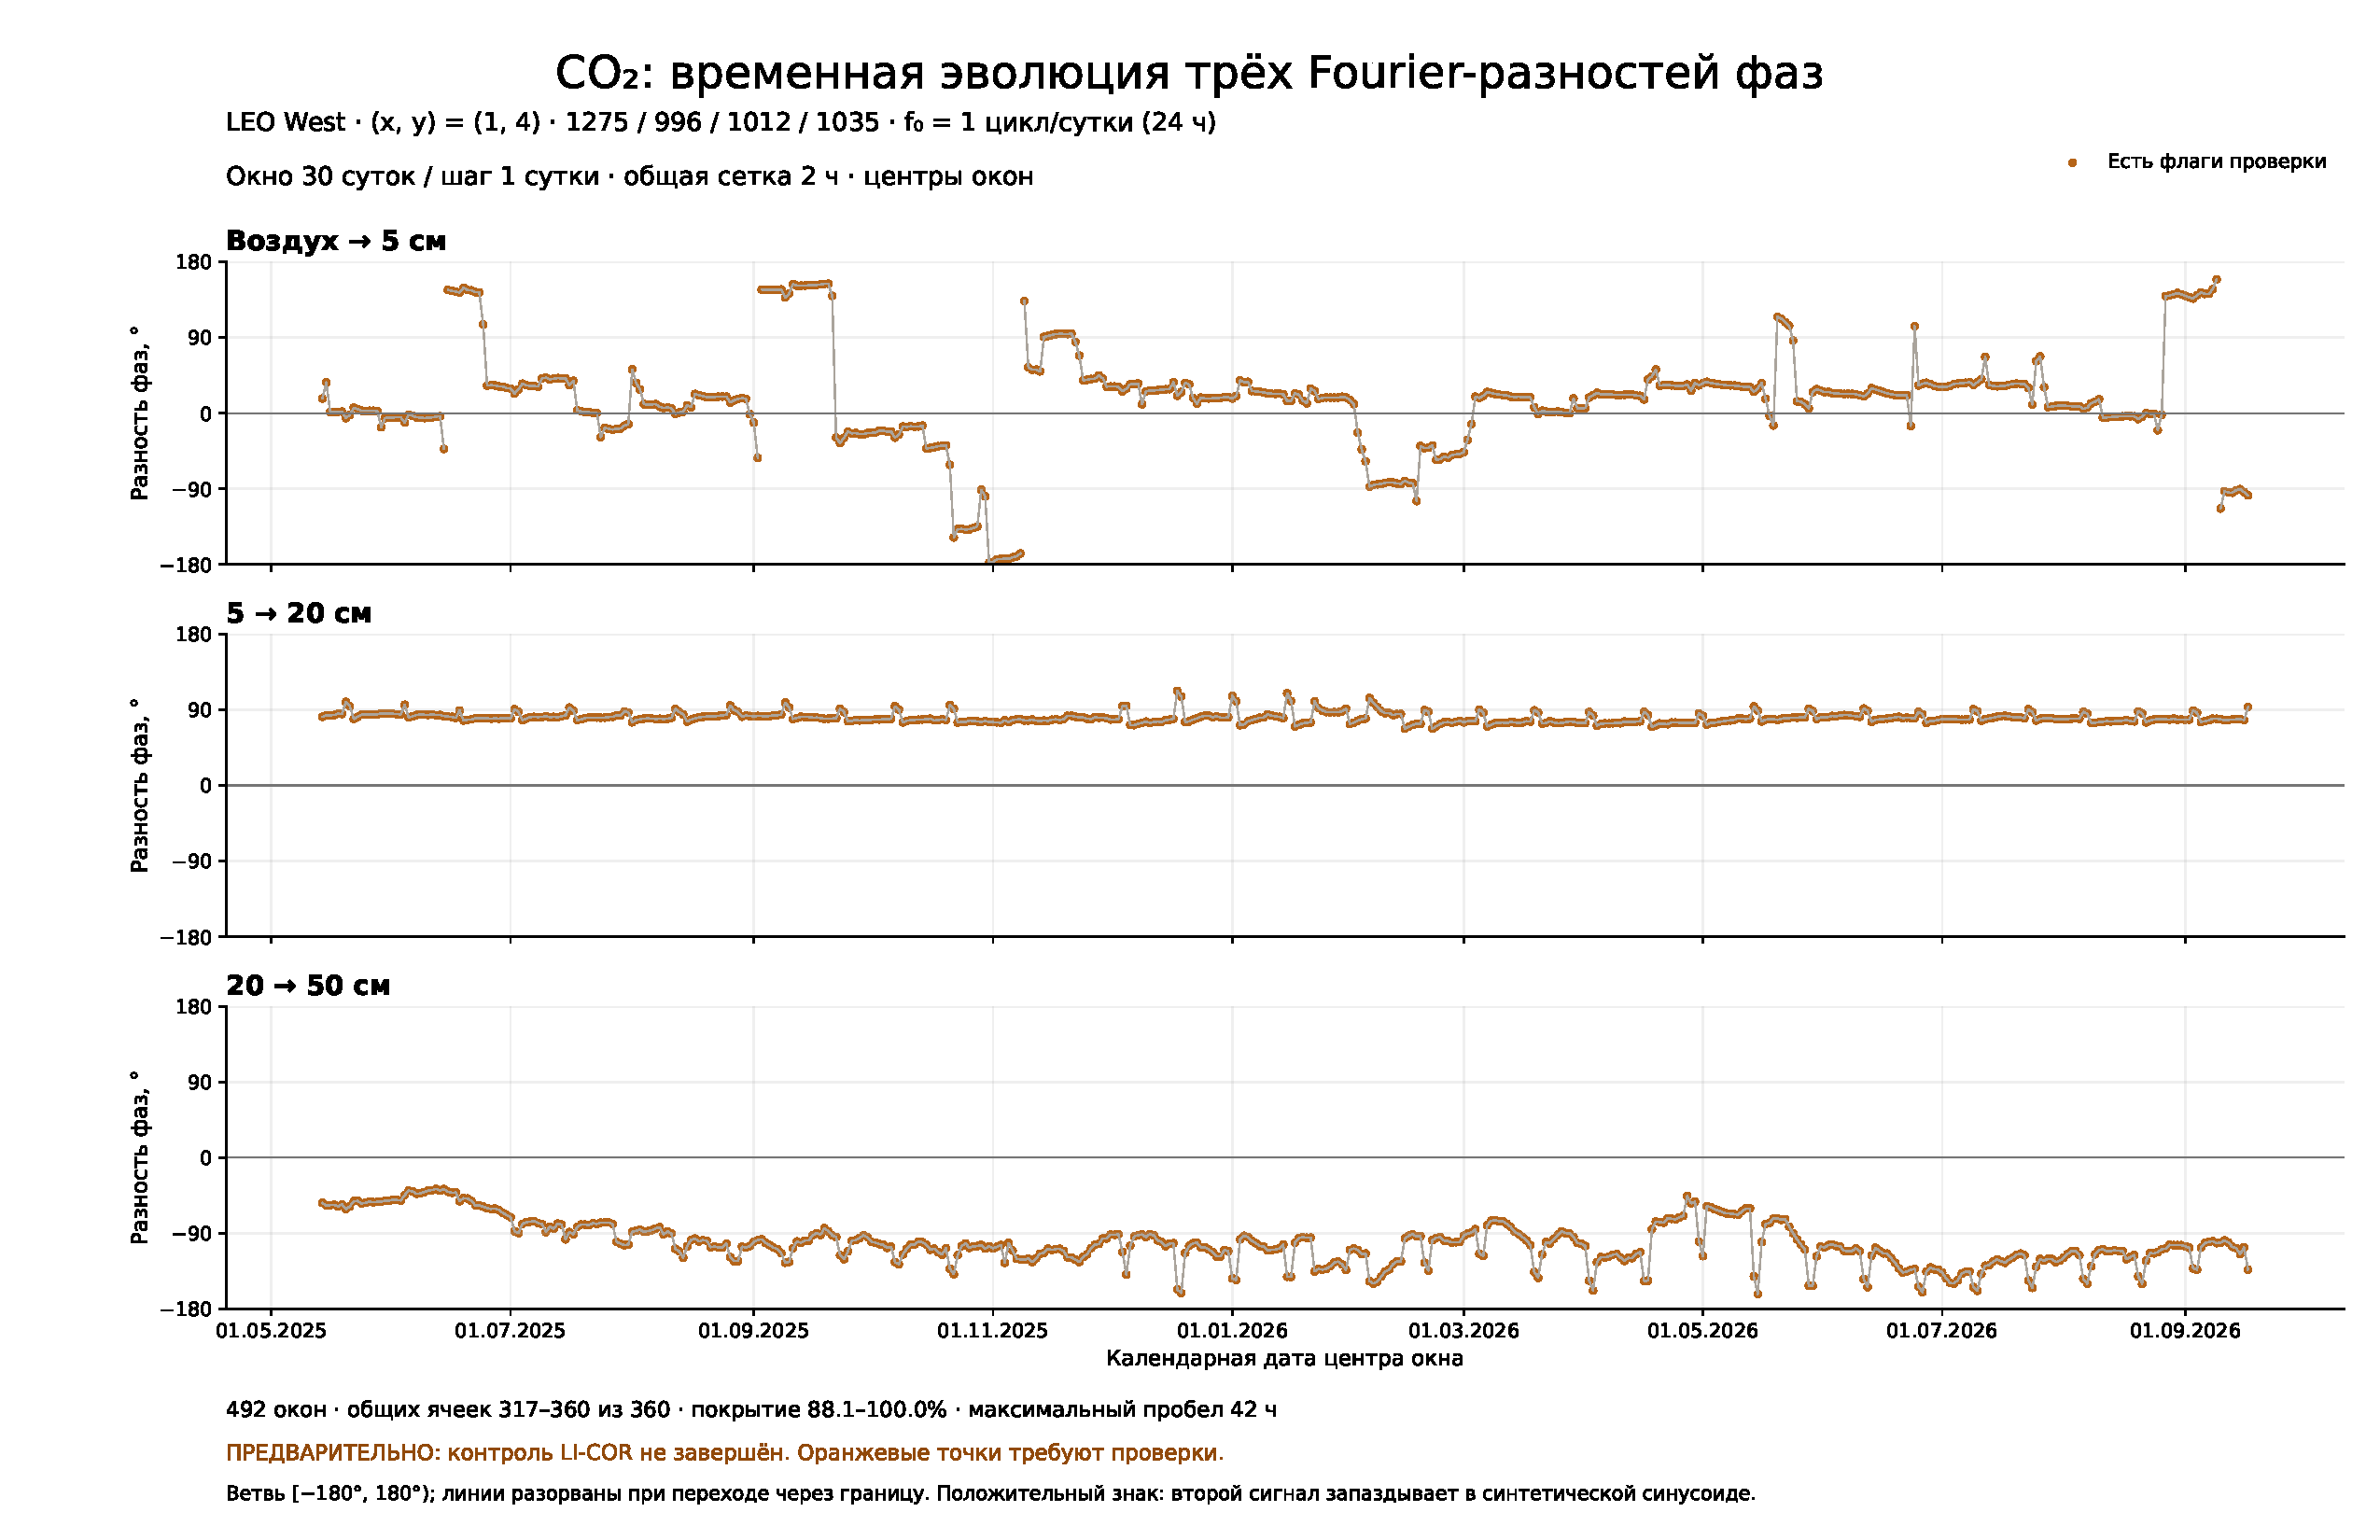
\includegraphics[width=.96\linewidth]{output/preliminary_fourier_phases/phase_evolution_17x11.pdf}
\caption{Pre-existing time evolution of three direct-Fourier relative phases, 30-day windows, one-day step, one cycle/day. Computed on the earlier input masks; not updated to the Stage~0.2 selected input.}
\label{fig:evolution}
\end{figure}
\end{landscape}
\begin{figure}[htbp]
\centering
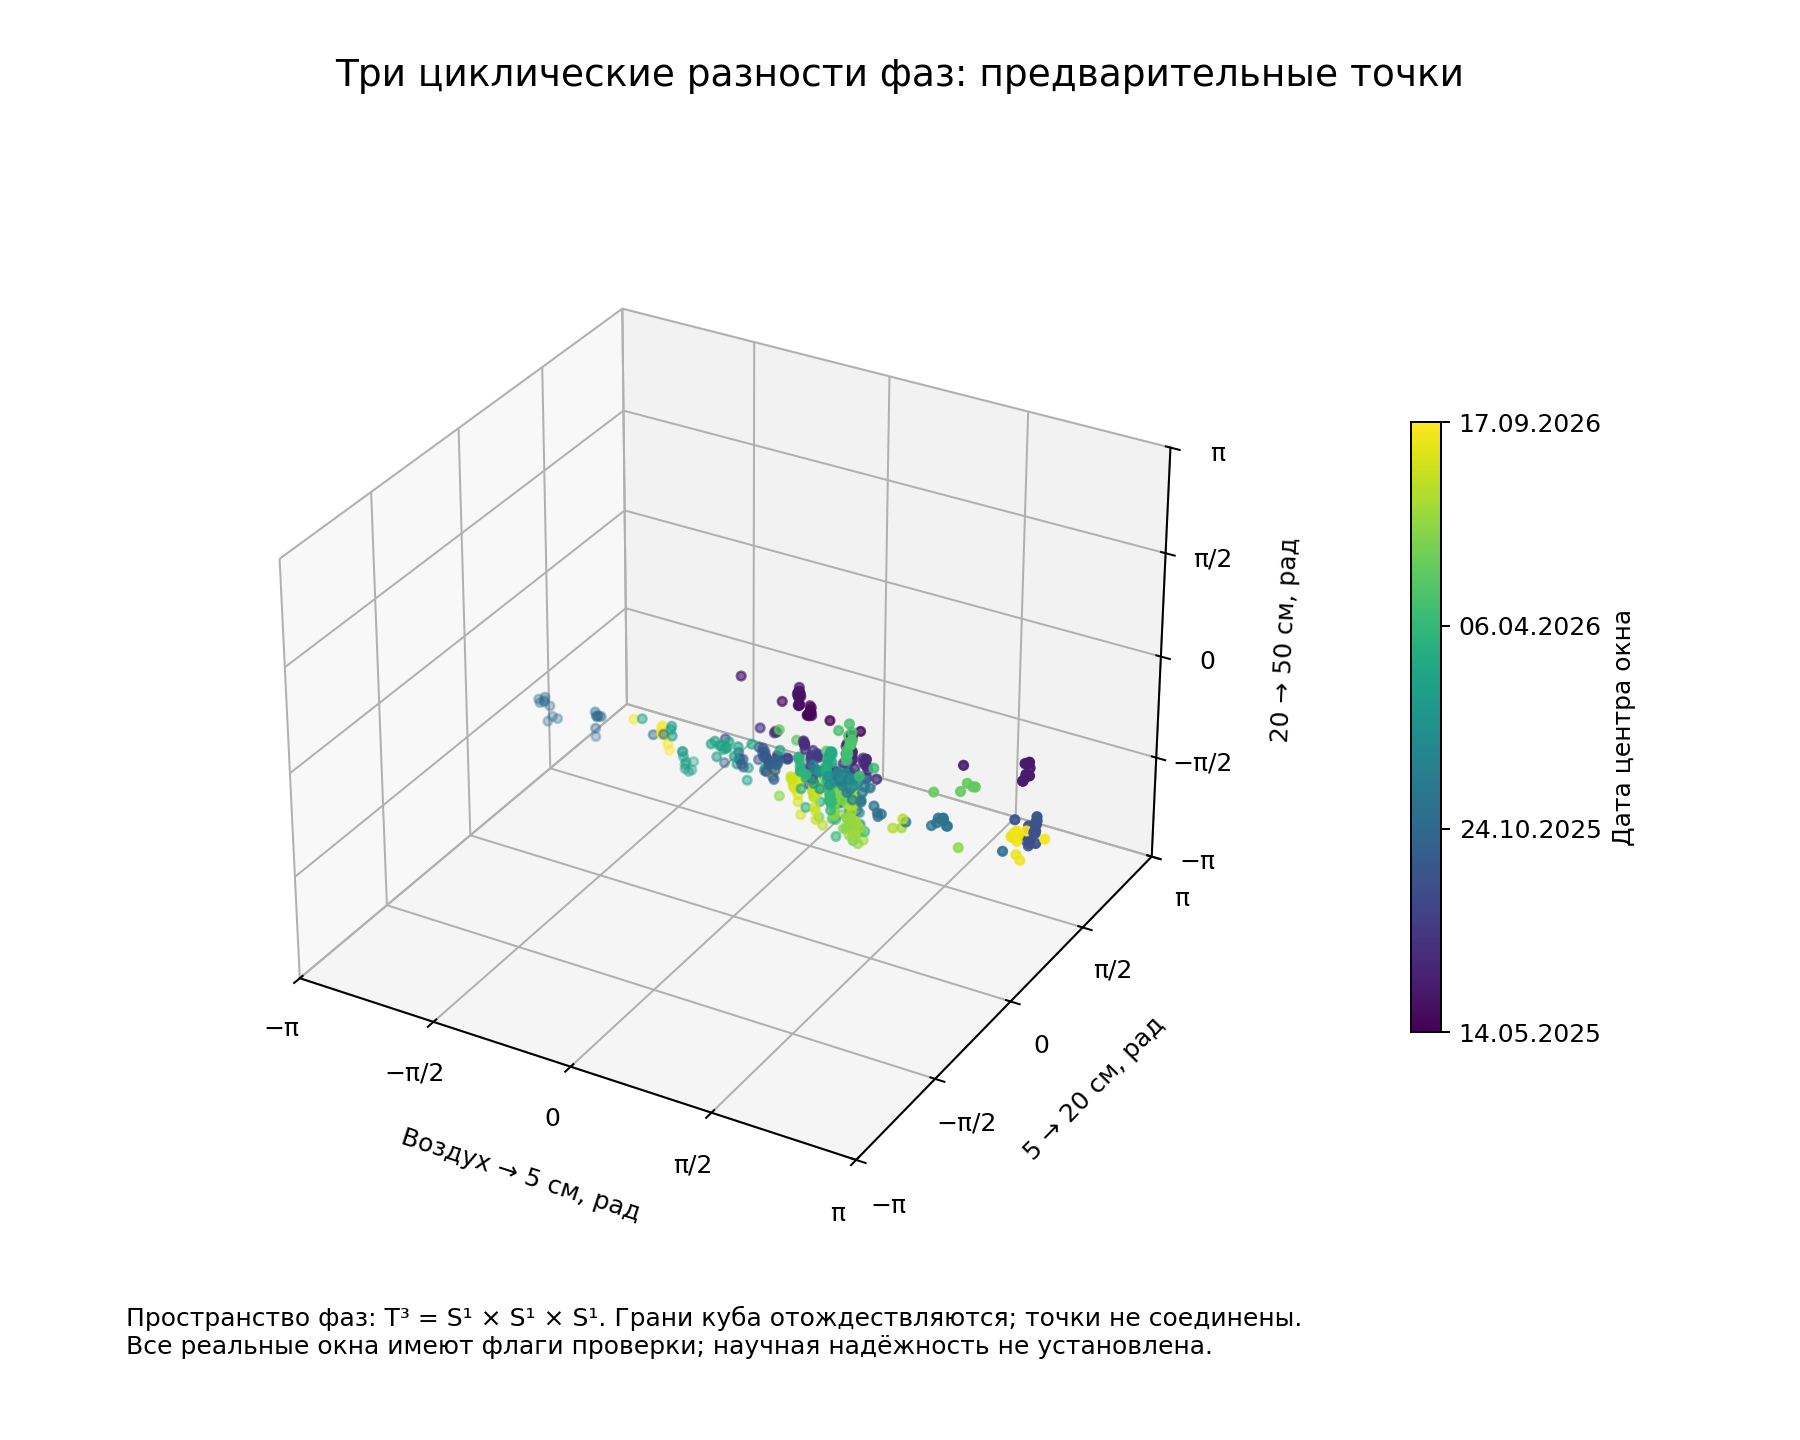
\includegraphics[width=.75\linewidth]{output/preliminary_fourier_phases/phase_trajectory_3d.png}
\caption{Pre-existing visualization of the three cyclic phase coordinates; it is not a demonstrated physical trajectory or a validated topological invariant.}
\label{fig:torus}
\end{figure}

\subsection{One 5-to-20 cm discontinuity examined for Stage 0.5/Q1}
\label{sec:jump}
My earlier 0.5/Q1 diagnostic selected a single adjacent pair by maximal absolute difference on the original $[-\pi,\pi)$ phase branch, with earlier occurrence breaking ties. The centers are 17.Dec.2025 and 18.Dec.2025, corresponding to 30-day windows from 02.Dec.2025 through 01.Jan.2026 and from 03.Dec.2025 through 02.Jan.2026, respectively. Neighboring windows overlap for 29 days and must not be treated as independent events. For the complex product $Q=F_5\overline{F_{20}}$, distinguish
\begin{equation}
d_Q=\wrap(\Arg Q_2)-\wrap(\Arg Q_1),\qquad
\delta_Q=\wrap(\Arg(Q_2\overline{Q_1})),\qquad
d_Q-\delta_Q=2\pi k,\ k\in\mathbb Z.
\label{eq:jump}
\end{equation}
The saved phases are $1.3815969902$ and $1.9625409175$ rad, so $d_Q=\delta_Q=+0.5809439273$ rad and $k=0$: \emph{this change is not an argument-branch crossing}. The coefficient argument changes are $+0.0891610601$ rad for $F_5$ and $-0.4917828672$ rad for $F_{20}$, agreeing with the product-phase increment. Their moduli decrease from 10.087605 to 6.749558 ppm and from 2.715018 to 2.004241 ppm. All eight neighboring windows have 360/360 common bins, but all contain review flags. None of these sampled coefficients is zero. There is no established amplitude-error threshold and no knowledge of an intervening continuous coefficient path, so a zero crossing cannot be proved or excluded. No physical event or mechanism is established \cite{phase,jump}.
\begin{figure}[htbp]
\centering
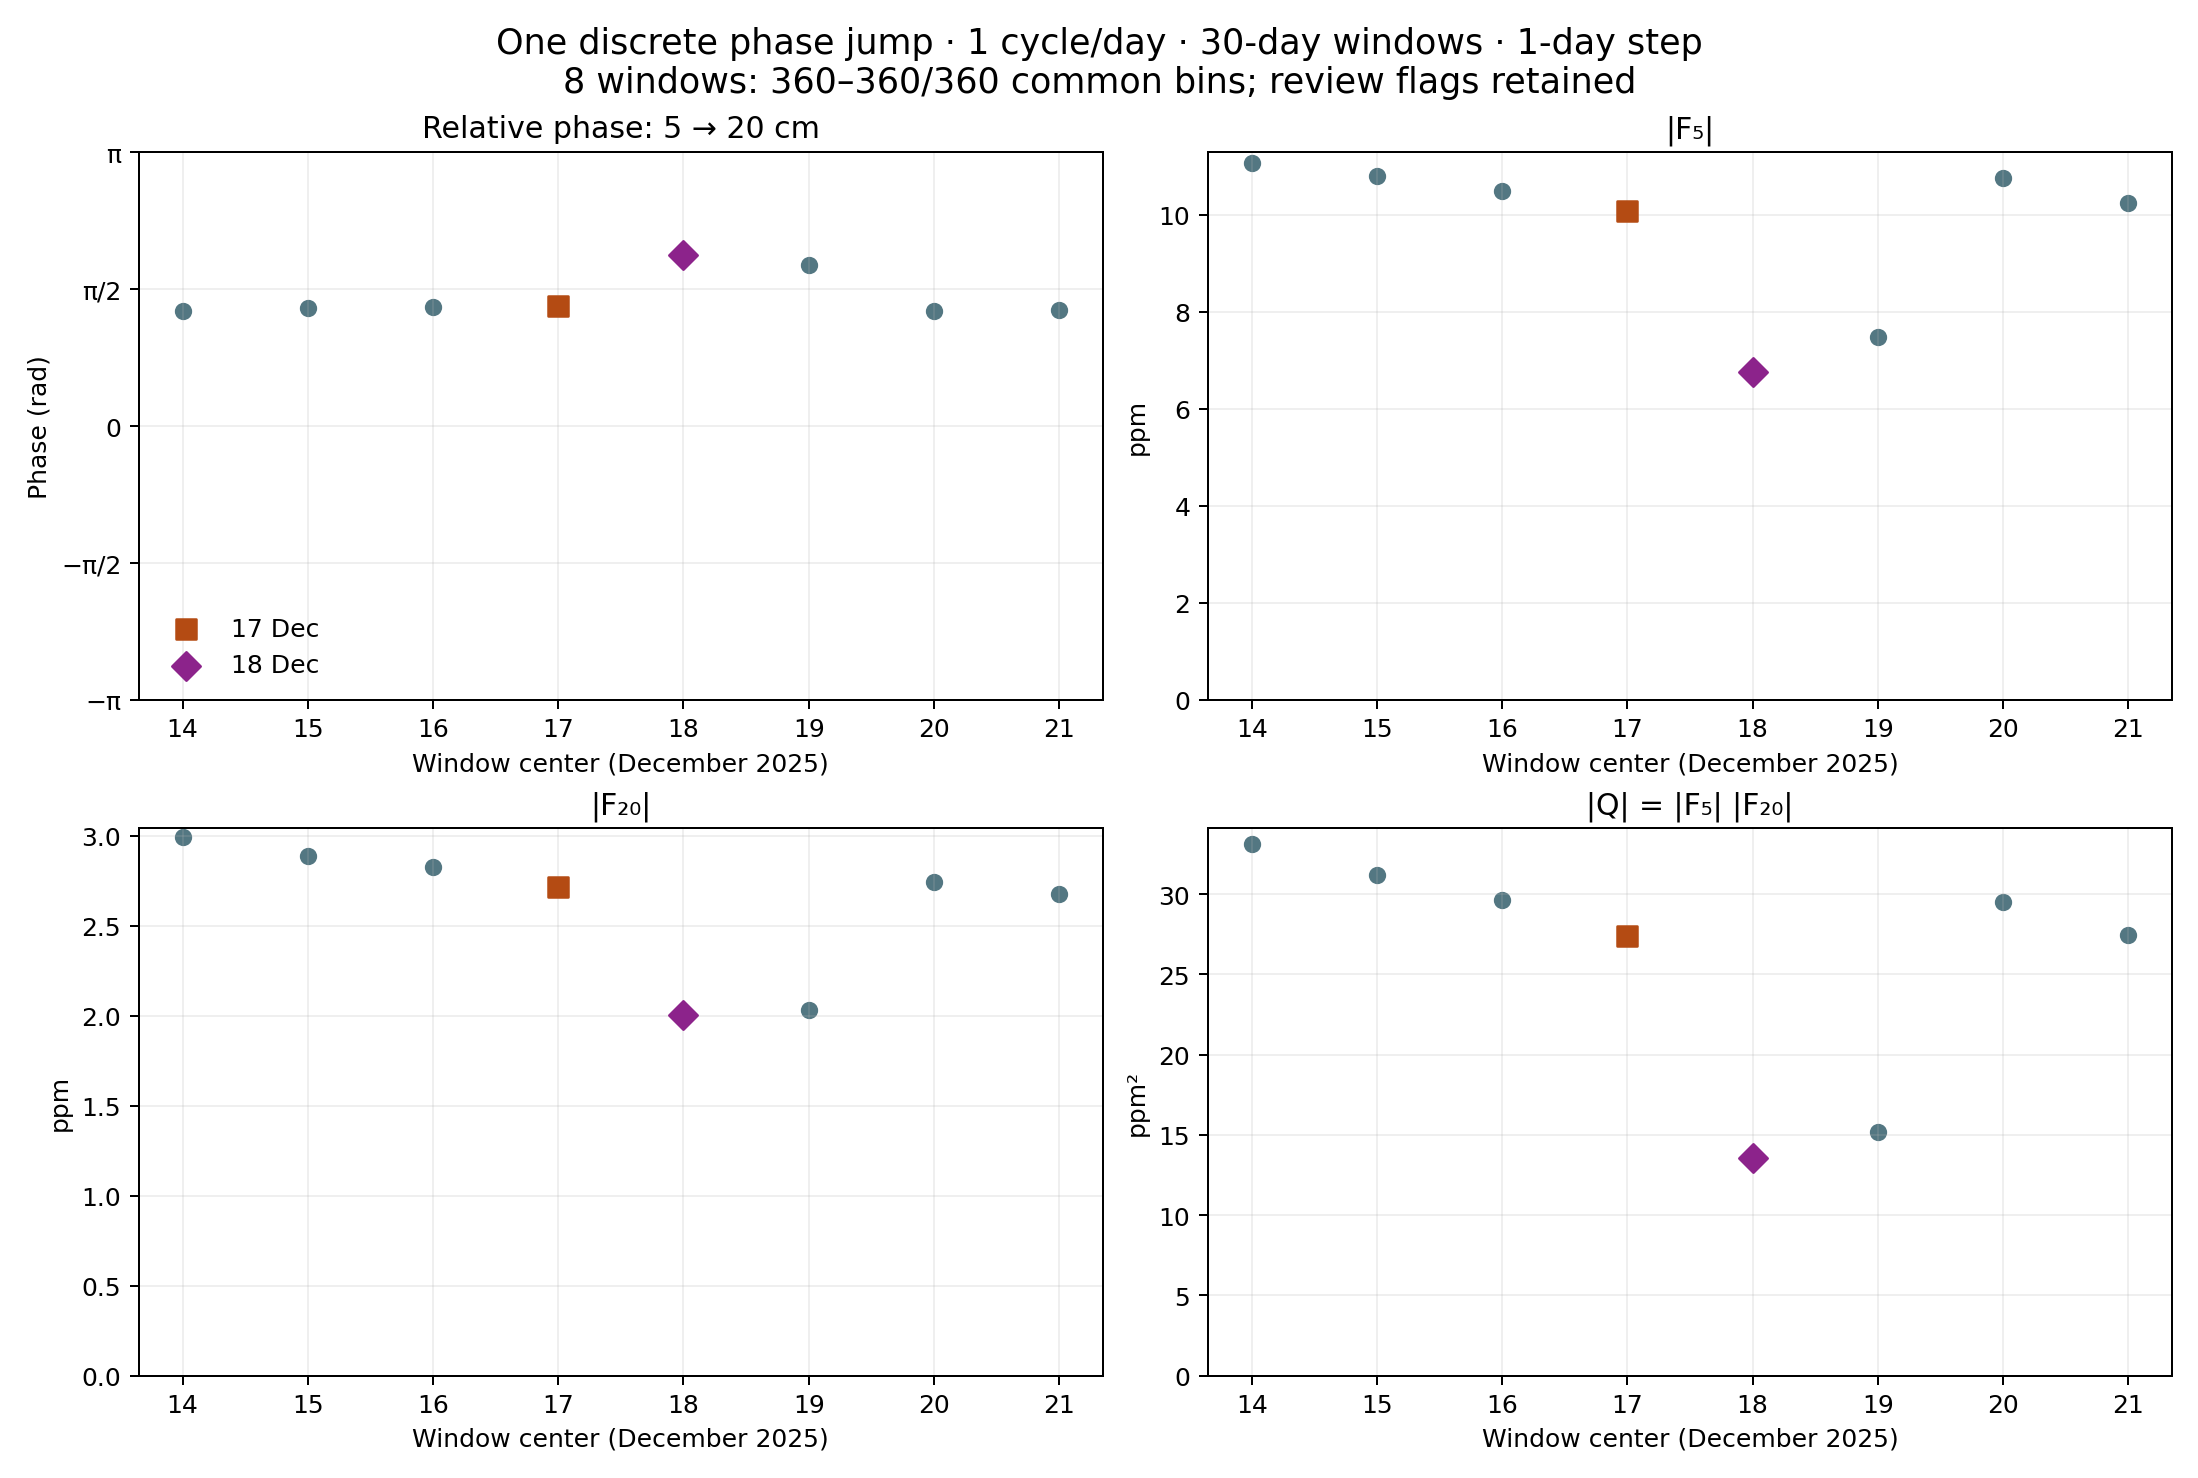
\includegraphics[width=.90\linewidth]{output/preliminary_fourier_phases/jump_diagnostic/phase_jump_local.png}
\caption{Saved discrete local relative phase and coefficient moduli around one selected phase change.}
\label{fig:jumplocal}
\end{figure}
\begin{figure}[htbp]
\centering
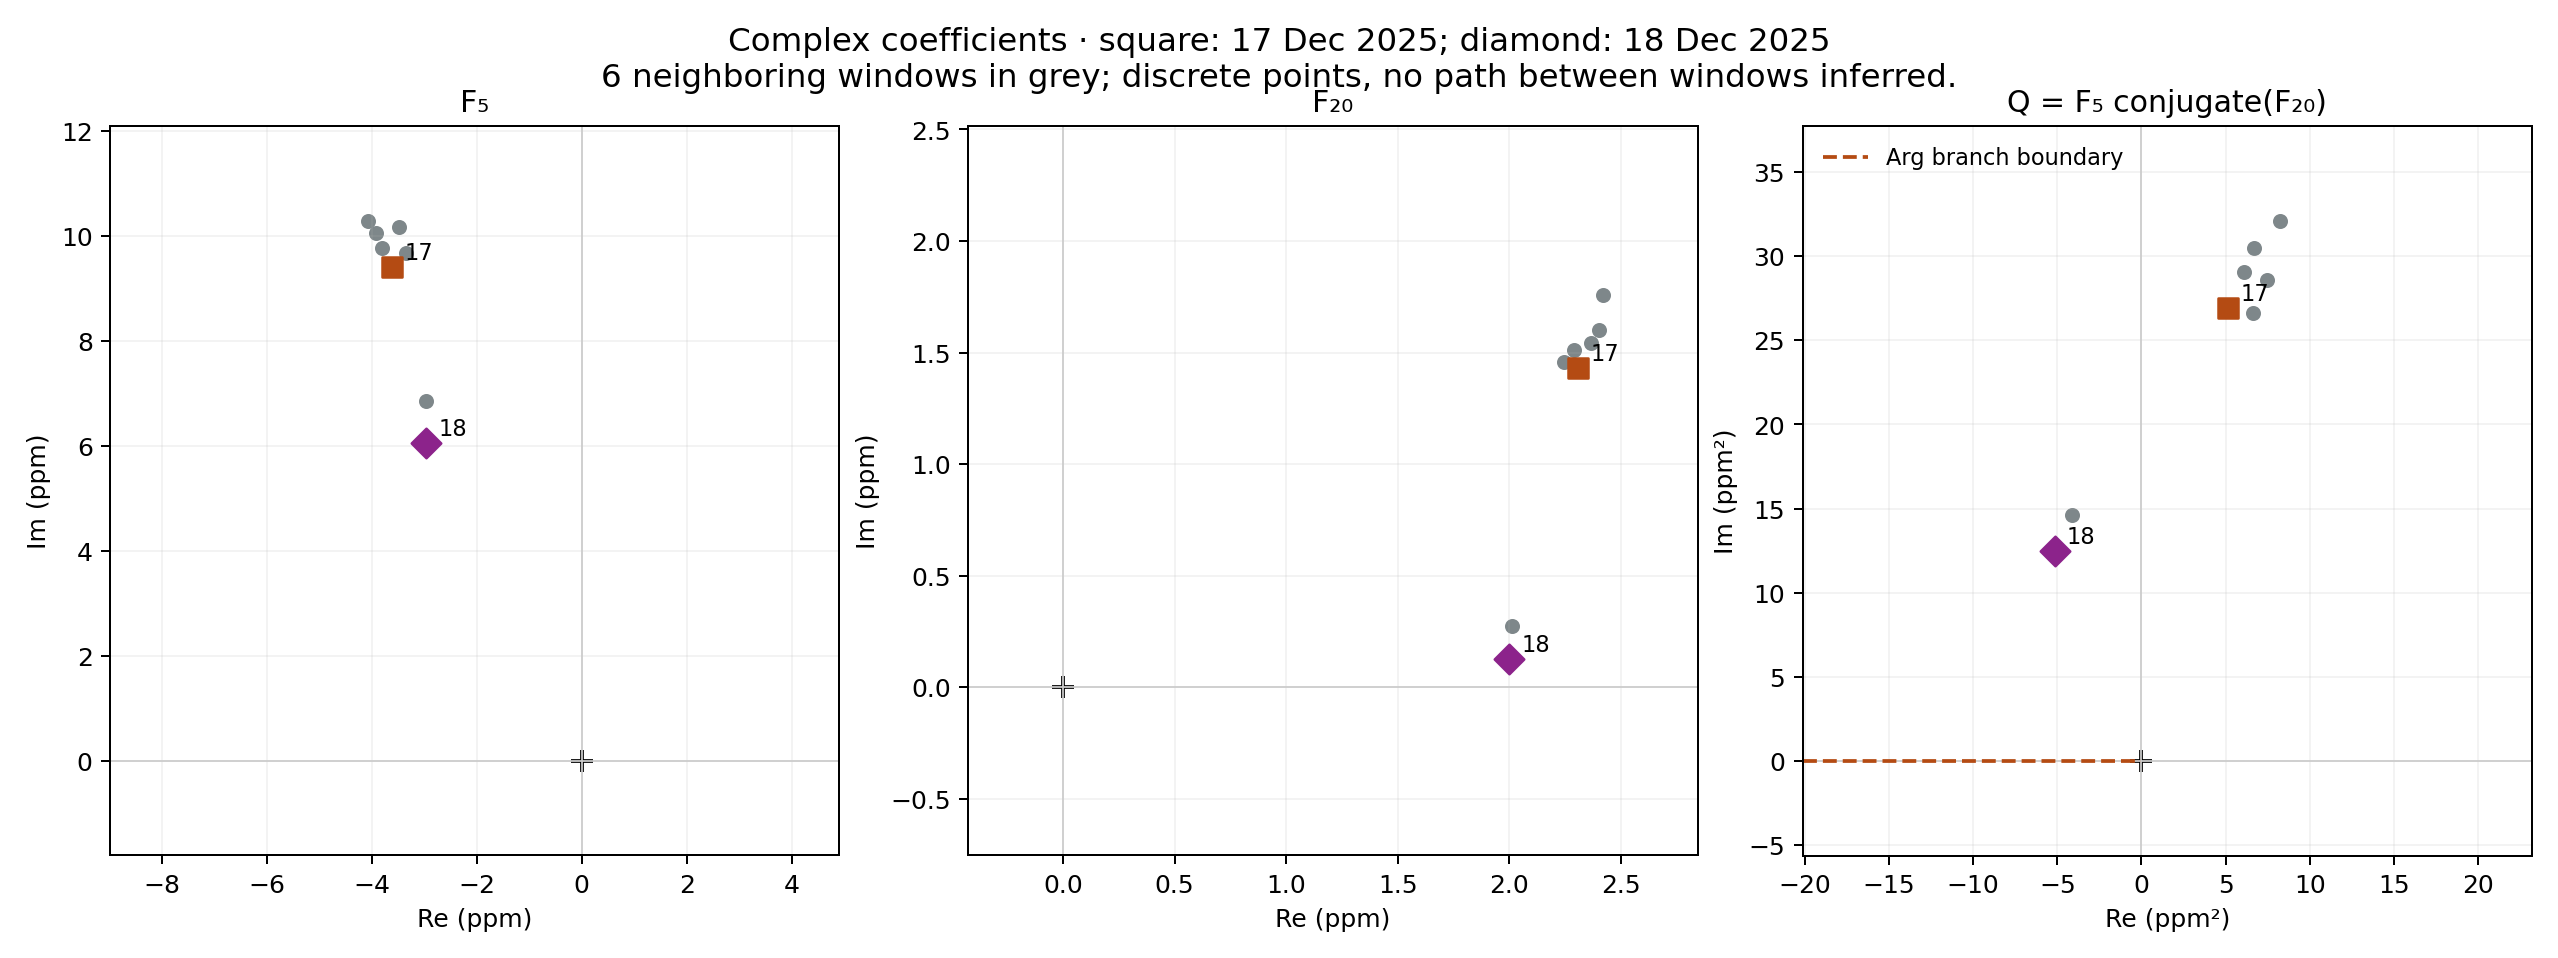
\includegraphics[width=.90\linewidth]{output/preliminary_fourier_phases/jump_diagnostic/phase_jump_complex.png}
\caption{Saved complex Fourier coefficients and their product $Q$, showing the origin and the relevant argument branch boundary without interpolating an unknown path.}
\label{fig:jumpcomplex}
\end{figure}

\subsection{Stage 0.5: sensitivity to 15-minute versus two-hour grids}
\label{sec:gridstudy}
After discussion with I.~R.~Gabitov on 23.Oct.2026,
I undertook one restricted diagnostic of the
\emph{subsurface} relative phases 5$\to$20~cm and
20$\to$50~cm. I used the accepted 17-month Stage~0.2
source observations, $f_0=1$ cycle/day, and matching
30-day windows stepped by one day.
I distinguished three supports:
(i) common 15-minute subsurface bins;
(ii) common two-hour subsurface bins;
(iii) two-hour subsurface means further restricted to
cells containing an actual atmospheric LI-COR reading.
This last operation is \emph{not} the same as aggregation,
and does not reconstruct a 15-minute air signal
\cite{gridpassport,gridvalidation}.

For the aggregation comparison I calculate the
cyclic difference
\begin{equation}
\delta_{u\to v}(W)=
\operatorname{Arg}\left[
\exp\left(i\left\{
\Delta\phi_{u\to v}^{(15\,\mathrm{min})}(W)
-\Delta\phi_{u\to v}^{(2\,\mathrm h)}(W)
\right\}\right)\right].
\label{eq:griddiff}
\end{equation}
I calculate an analogous circular difference between
the unrestricted two-hour subsurface phase and the
phase on two-hour cells also occupied by air. All
\textbf{489 windows} yielded finite paired estimates
for both subsurface depth pairs in all three variants.

\begin{center}
\small
\begin{tabular}{@{}llrrr@{}}
\toprule
Effect & Pair & Median $|\delta|$ & 95th pct.\ $|\delta|$ & Maximum $|\delta|$\\
\midrule
15 min -- 2 h & 5$\to$20 cm & 0.010179 & 0.050569 & 0.080158\\
15 min -- 2 h & 20$\to$50 cm & 0.050098 & 0.154327 & 0.317131\\
Air support & 5$\to$20 cm & 0.011741 & 0.315633 & 0.430516\\
Air support & 20$\to$50 cm & 0.052175 & 0.297058 & 0.399709\\
\bottomrule
\end{tabular}
\end{center}
All values are in radians. The 15-minute subsurface
windows have 2,776--2,831 occupied common cells
out of 2,880 possible; two-hour subsurface support
has 360/360, and the two-hour support additionally
restricted by air has 316--360/360. The respective
longest missing common-cell intervals are 1, 0 and
42 hours. The preserved validation records
\textbf{26 passing tests}, including seven new narrow
checks; it does not establish physical uncertainty
or a new acceptance threshold.

\begin{figure}[htbp]
\centering
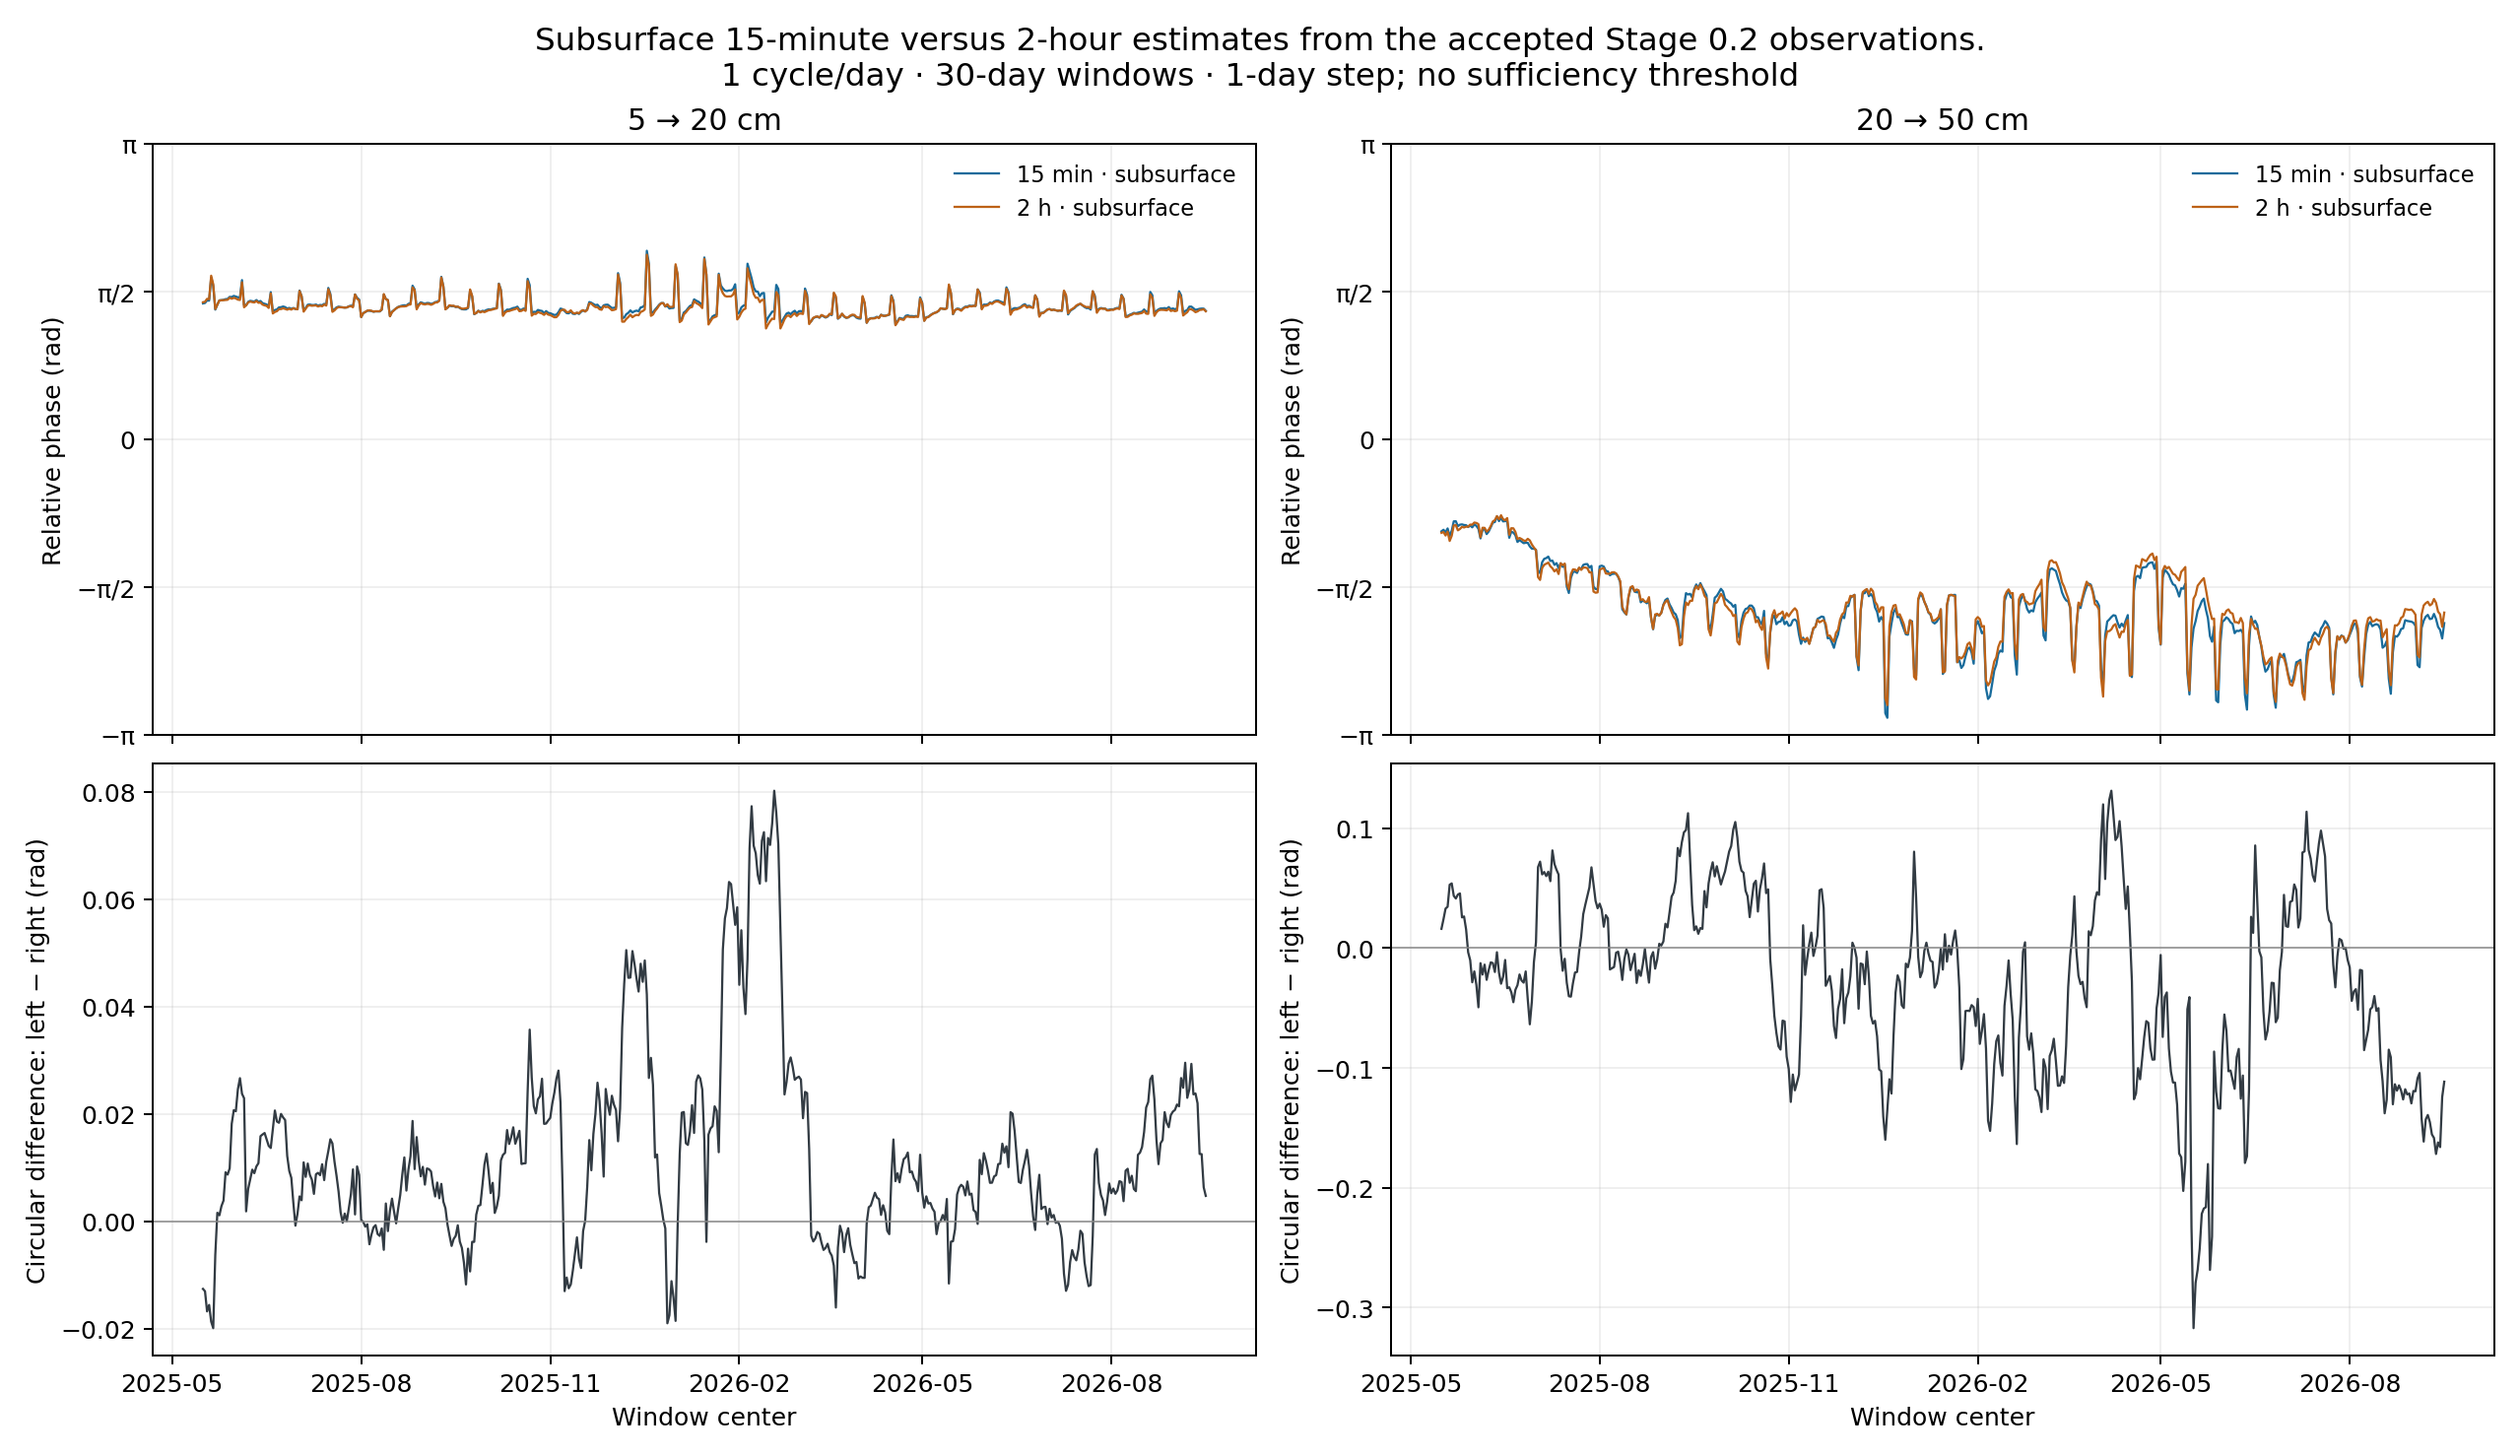
\includegraphics[width=.95\linewidth]{output/preliminary_fourier_phases/grid_resolution/grid_aggregation.png}
\caption{Existing comparison between actual subsurface
15-minute and two-hour Fourier phases on the same
accepted measurements. The lower panels show circular
differences between estimates, not errors relative
to an unknown true phase.}
\label{fig:gridaggregation}
\end{figure}

\begin{figure}[htbp]
\centering
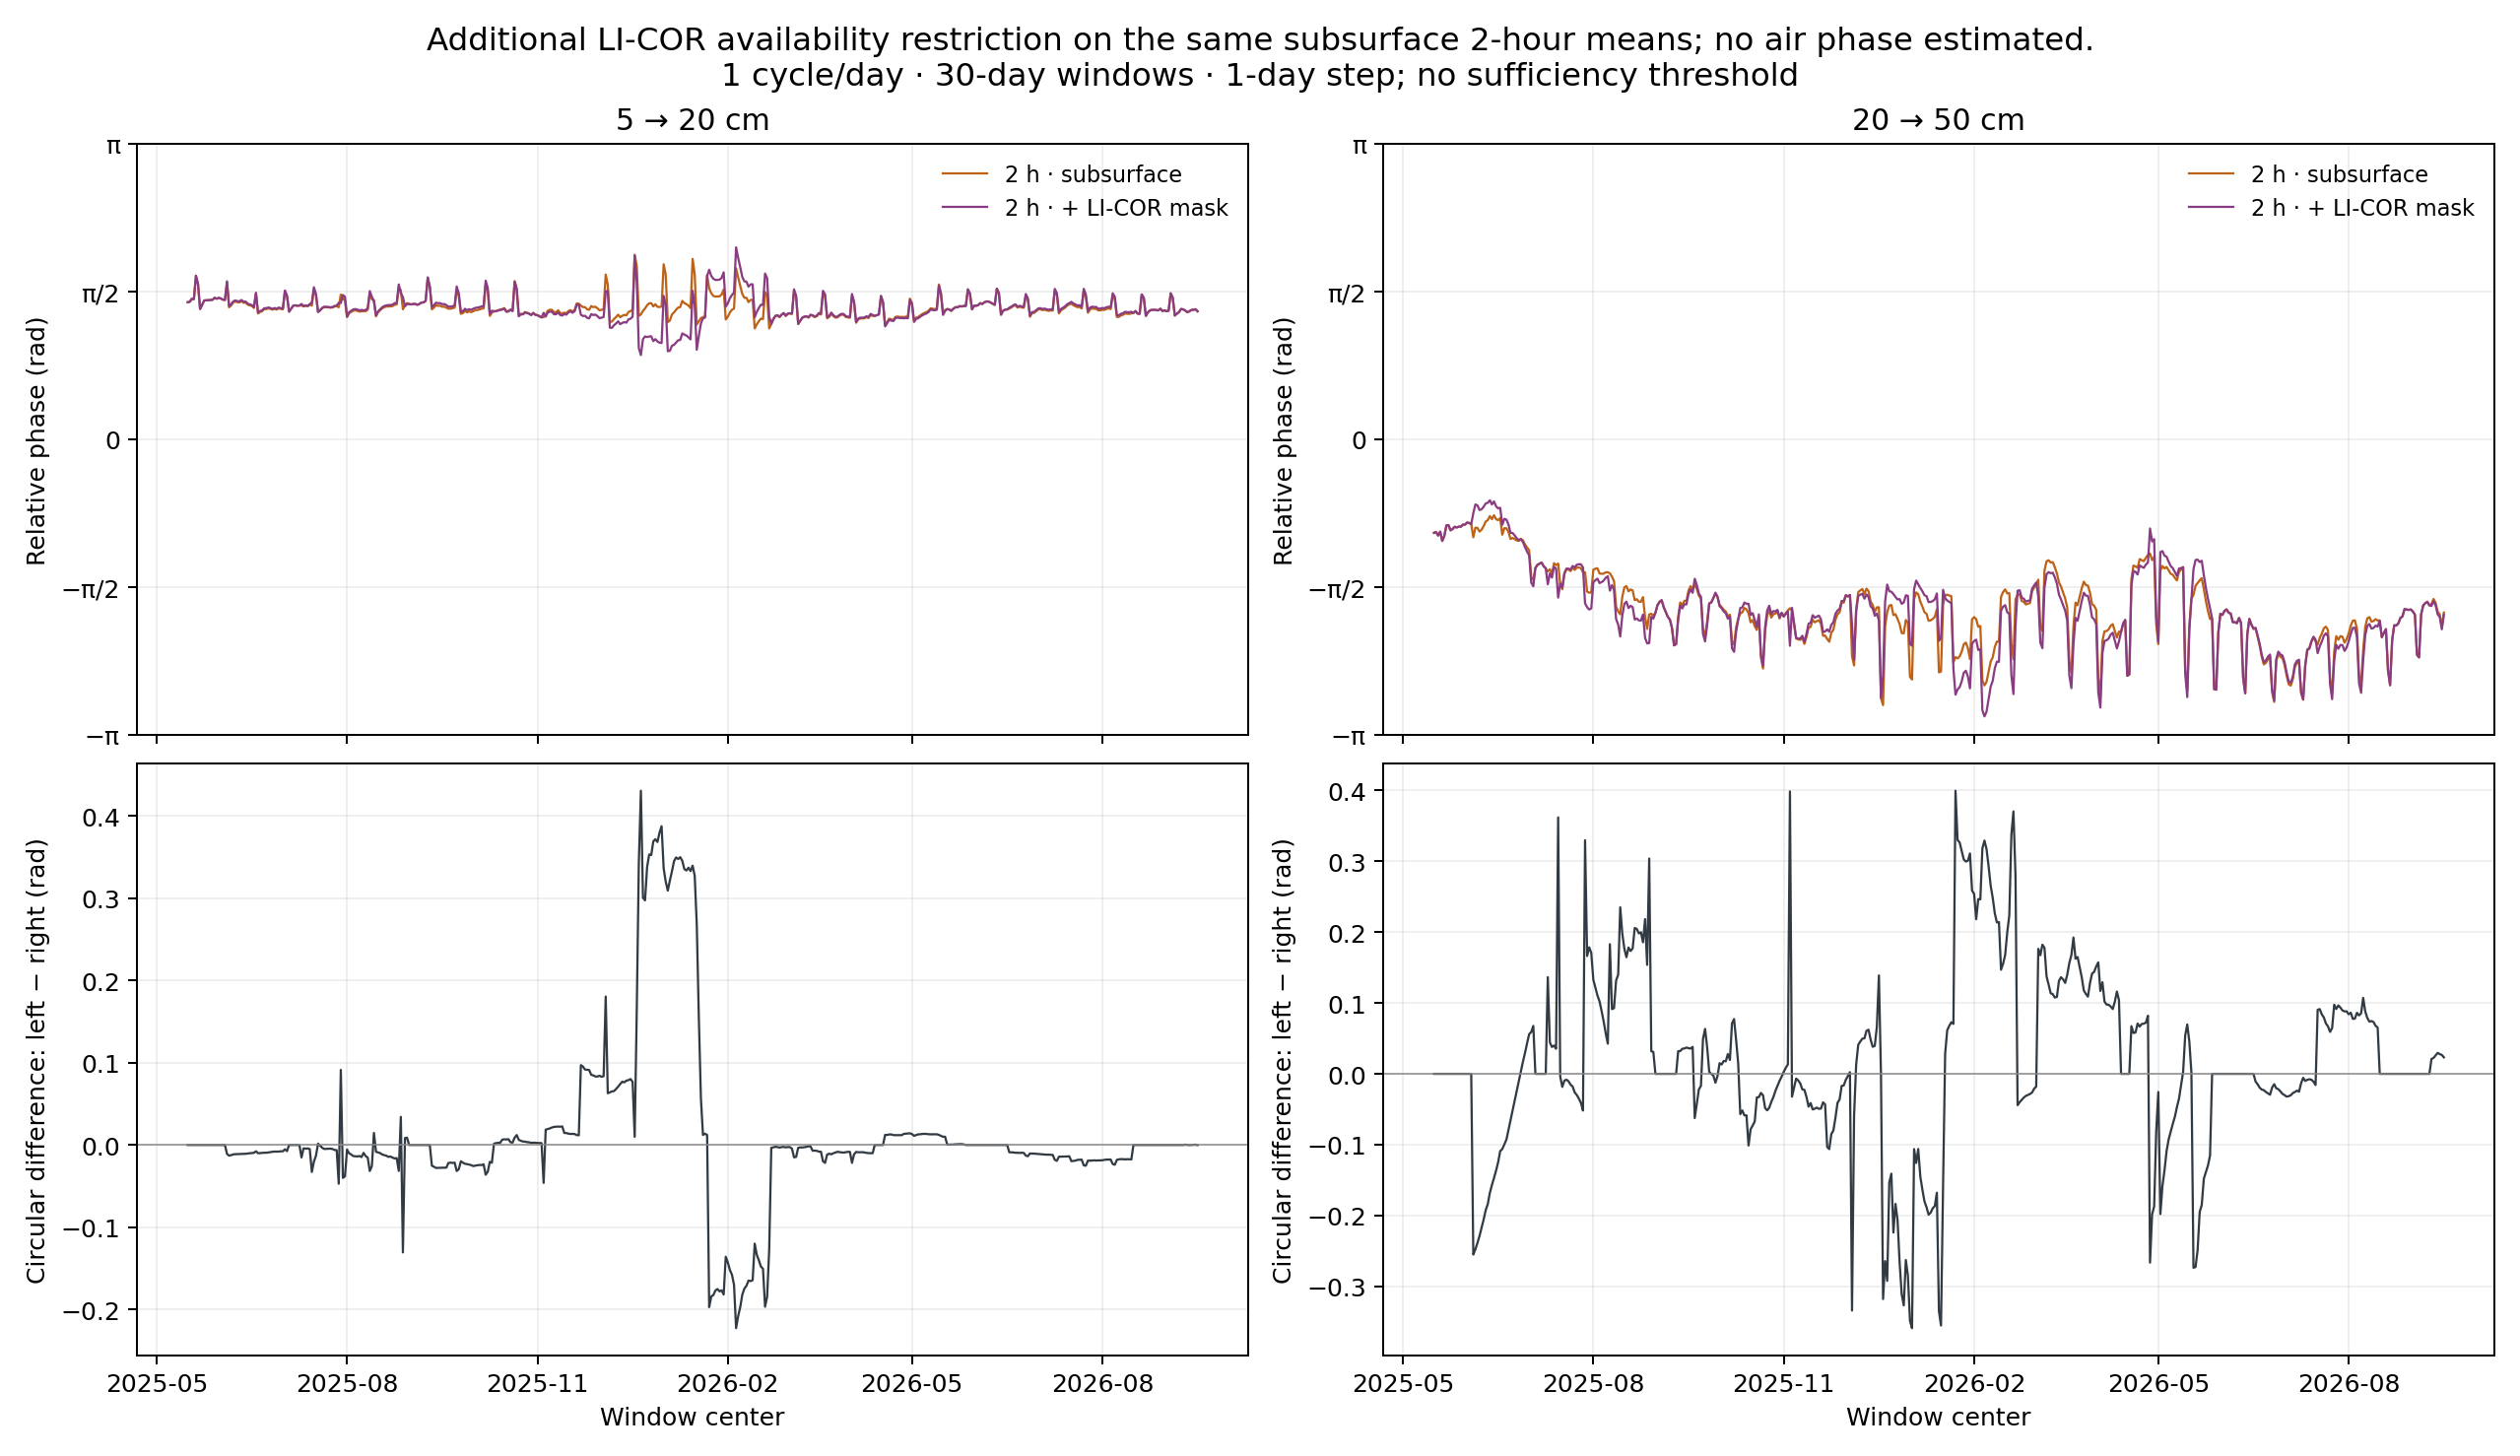
\includegraphics[width=.95\linewidth]{output/preliminary_fourier_phases/grid_resolution/grid_air_support.png}
\caption{Existing effect of restricting two-hour
subsurface support by atmospheric LI-COR availability.
The two-hour subsurface means themselves are preserved;
this is not a 15-minute atmospheric phase analysis.}
\label{fig:gridair}
\end{figure}

\begin{figure}[htbp]
\centering
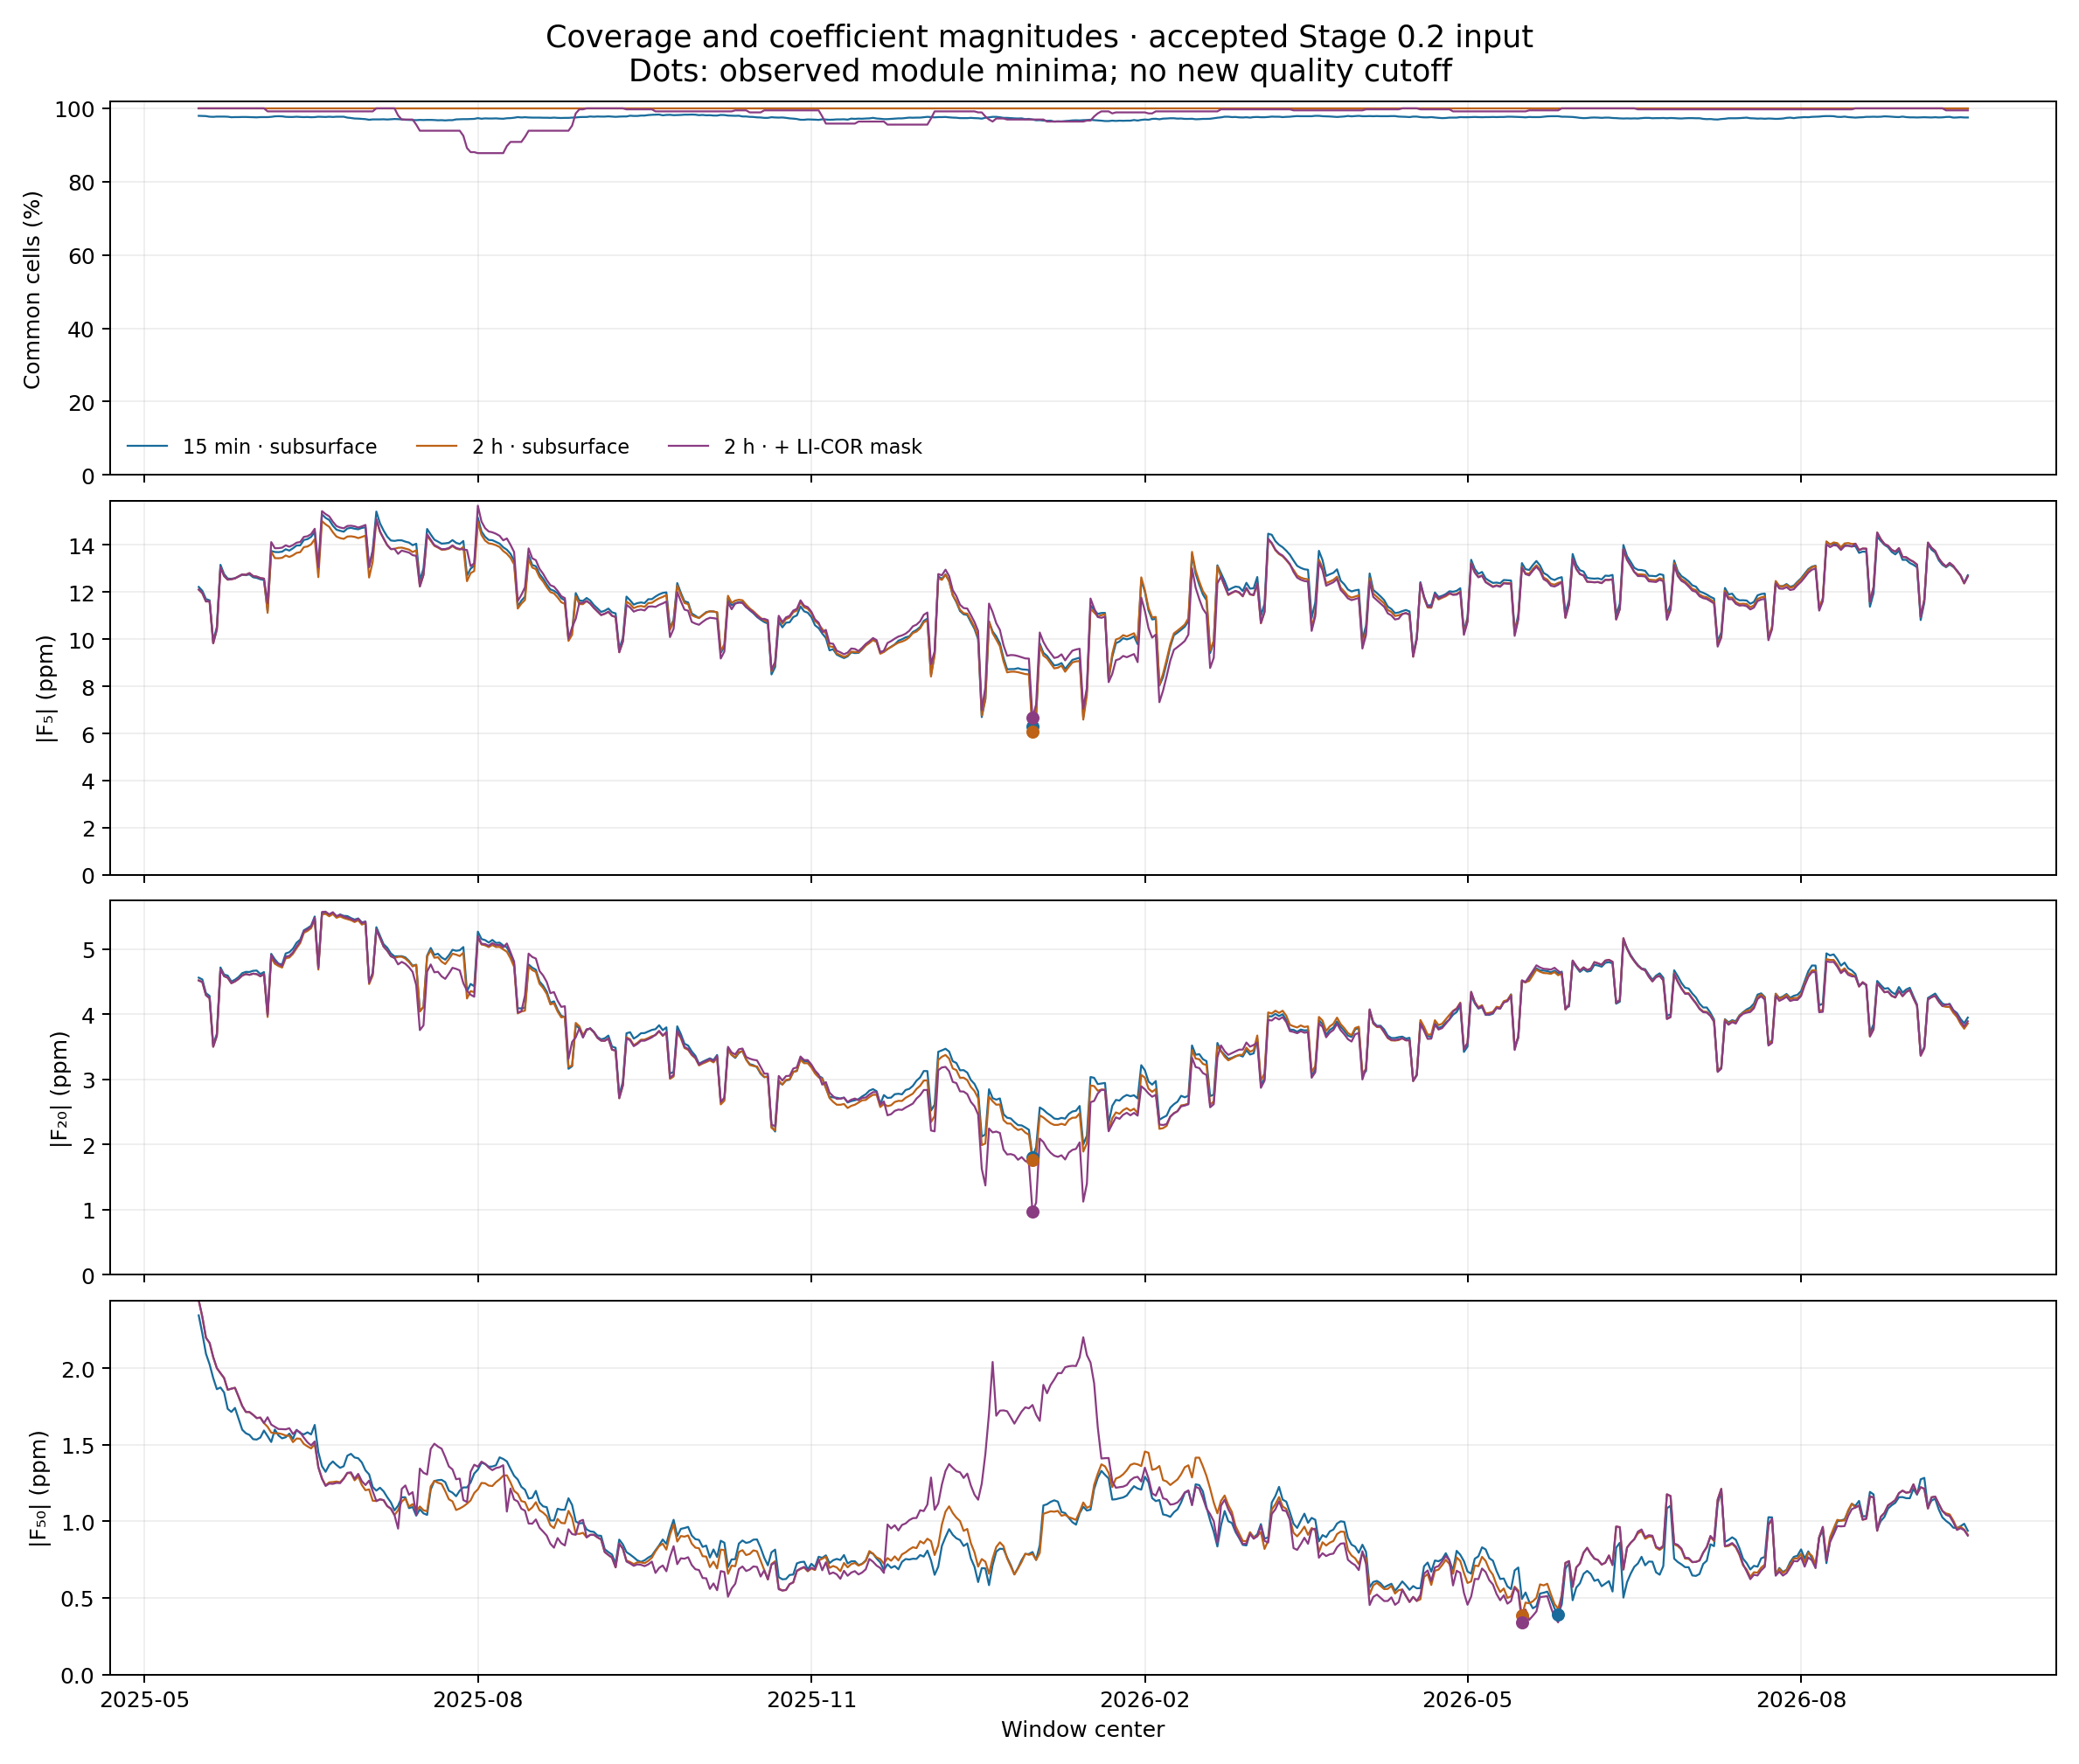
\includegraphics[width=.95\linewidth]{output/preliminary_fourier_phases/grid_resolution/grid_context.png}
\caption{Existing coverage and Fourier-coefficient
moduli by grid variant. Low extrema and missingness
are shown descriptively; no new admissibility
threshold is introduced.}
\label{fig:gridcontext}
\end{figure}
I interpret this calculation as a check of sampling
and common-support sensitivity for two subsurface
pairs at one daily frequency. Overlapping windows
are not independent observations. The sufficiency
of two-hour resolution remains a matter for an
explicit methodological decision by I.~R.~Gabitov.

\section{Historical analyses, not spectral-phase evidence}
\label{sec:historical}
In my earlier Chapter 1, I fitted a fixed diurnal harmonic. My earlier Chapter 2 studied the different West vertical W\_R4\_C-4 from 11.Sep.2013 through 30.Sep.2026, over 157 months and 2,614,638 archived raw measurements. Its final historical processing retained 43 jointly admitted months, 23 vectors of absolute daily maximum times $H(d)$ and 25 daily-amplitude vectors $A(d)$. These are not four-channel spectral-window admissions. My earlier Chapter 3 found no established reproducible long-term evolution under its original absolute-maximum-time and amplitude procedure. The historical input and its limitations are retained but are not recalculated or interpreted as either confirming or refuting the new relative spectral-phase problem \cite{readme,historical}.

\section{Mathematical validation and physical interpretation}
\label{sec:validation}
I treat the argument of a nonzero complex Fourier
coefficient as a computed angular coordinate, not
automatically as a reliable physical travel time.
In particular, small moduli can make phase sensitive
to perturbation, and changing the common observation
support can change the result. The single older Q1
jump and the new grid-resolution diagnostic test
different mathematical issues. Neither establishes
a CO$_2$ transport mechanism.

For subsequent physical interpretation, the PLAN
records an elementary one-dimensional diffusion
hypothesis discussed with I.~R.~Gabitov on
23.Oct.2026:
\begin{equation}
\frac{\partial C}{\partial t}
=D\frac{\partial^2 C}{\partial x^2},\qquad D>0,
\label{eq:diffusion}
\end{equation}
where $x$ is depth directed downward.
This has not been fitted or validated for LEO.
A possible, not yet established, extension is
\begin{equation}
\partial_t C=
\partial_x\bigl(D_{\rm eff}(\theta,x,t)\partial_xC\bigr)
+S(x,t),
\label{eq:diffusionwet}
\end{equation}
where moisture $\theta$, transport coefficient
$D_{\rm eff}$ and combined source/sink term $S$
require their own definitions and measurements.
Any physical balance must additionally account for
the choice of concentration variable and pore-gas
storage. Candidate idealized boundary conditions
discussed with I.~R.~Gabitov are
\begin{equation}
-D_{\rm eff}\,\partial_x C(0,t)
=k[C_{\rm air}(t)-C(0,t)],\qquad
\partial_x C(L,t)=0.
\label{eq:bc}
\end{equation}
The surface Robin condition is not automatically
equivalent to my separate observational assumption
$C_0(t)=C_{\rm air}(t)$.
I keep them distinct pending a physical model.

With $\tau=t/T_0$ and $y=x/X_0$ the constant-$D$
reference equation becomes
\begin{equation}
\partial_\tau C=
\frac{DT_0}{X_0^2}\partial_y^2C,\qquad
T_0=\frac{X_0^2}{D_0}\quad(D=D_0>0).
\label{eq:scale}
\end{equation}
The illustrative length $X_0=0.1$~m
does not supply a numerical $T_0$ without $D_0$;
the scale is not a measured phase delay.
None of these models starts future Chapter~6
or implies an estimate of biological activity
or chemical interaction \cite{plan,maier}.

\section{Buchstaber framework: approved methodological preparation only}
\label{sec:buchstaber}
The separate existing Chapter 4 notebook states that application to LEO has not begun. For an admissible uniform scalar series $(f_1,\ldots,f_N)$, the proposed unfolding consists of
\begin{equation}
X_k=(f_k,\ldots,f_{k+n-1})^\mathsf{T}\in\mathbb R^n,\quad
P=N-n+1,\quad k=1,\ldots,P.
\end{equation}
Writing $\bar X=P^{-1}\sum_kX_k$ and $S=P^{-1}\sum_k(X_k-\bar X)(X_k-\bar X)^\mathsf T$, with eigenvalues $\lambda_1\geq\cdots\geq\lambda_n\geq0$, the quadratic affine projection identity is
\begin{equation}
E_q=\min_{\dim L=q}\frac1P\sum_k\|(I-\Pi_L)(X_k-\bar X)\|_2^2
=\sum_{i=q+1}^n\lambda_i,\qquad L_q^*\in G(n,q).
\end{equation}
This standard mathematical identity is not a measured LEO result. In particular the Grassmannian $G(n,q)$ is not the phase torus $\mathbb T^3$. Synthetic tests, validated data and a separately approved protocol are prerequisites for application to LEO \cite{buchnotebook,buch1994,buch2025}.

\section{Limitations and open questions}
\label{sec:limits}
My accepted 0.2 data scope and limited 0.1-B
hydrology do not establish a complete operational
irrigation-event calendar. The 37 wetting dates
provide coarse indirect environmental markers,
not exact known forcing times. The earlier 0.3/0.4
illustrations are retained on their old input masks.
I have not recomputed the three four-channel phase
series for the newly accepted 489-window view.
The later 15-minute/two-hour study tests only two
subsurface pairs, not a 15-minute atmospheric
signal. I have not adopted a cutoff declaring
two-hour sampling sufficient, or quantified error
against a known true phase. Overlapping windows
are dependent and coefficient moduli and real gaps
may limit interpretation. The partial Arevalo et al.
precipitation dataset does not replace a full
operational log. No diffusion coefficient or
transport, chemical or biological source has
been identified from these observations
\cite{plan,hydroaudit,gridpassport}.

\section{Next approved steps}
\label{sec:next}
I remain at Stage~0.5 before new Chapter~1.
The approved immediate discussion with
I.~R.~Gabitov must present the original
amplitude spectra, the three preliminary temporal
phase series, the 0.5/Q1 example, the accepted
17-month input, hydrological coverage and 37
wetting-day markers, and the new two-pair
temporal-resolution diagnostic.
The open decision is whether two-hour sampling
is sufficient for the selected daily spectral
phase question, with explicit consideration of
the remaining irrigation-log gaps and the
chosen frequency, window, step and phase
assessment protocol. I do not automatically
launch 15-minute atmospheric reconstruction,
machine learning, additional frequencies or
physical modeling, or mark Chapter~1 as begun.
The independent Buchstaber preparation is
not evidence of its application to LEO.

\section*{Sources, figures and reproducibility}
\addcontentsline{toc}{section}{Sources, figures and reproducibility}
This report consolidates the source repository at commit \texttt{5fb1ca89260192f189d69ac73fa360caec7598d5}, 28.Oct.2026. The existing figures used here, without regeneration, are:
\begin{itemize}
\item \texttt{output/stage01\_irrigation/pilot\_hydrology\_17months.png};
\item \texttt{output/preliminary\_fourier\_phases/grid\_resolution/grid\_aggregation.png};
\item \texttt{output/preliminary\_fourier\_phases/grid\_resolution/grid\_air\_support.png};
\item \texttt{output/preliminary\_fourier\_phases/grid\_resolution/grid\_context.png};
\item \texttt{output/preliminary\_spectra/four\_channel\_spectra\_17x11.pdf};
\item \texttt{output/preliminary\_fourier\_phases/phase\_evolution\_17x11.pdf};
\item \texttt{output/preliminary\_fourier\_phases/phase\_trajectory\_3d.png};
\item \texttt{output/preliminary\_fourier\_phases/jump\_diagnostic/phase\_jump\_local.png};
\item \texttt{output/preliminary\_fourier\_phases/jump\_diagnostic/phase\_jump\_complex.png}.
\end{itemize}
I preserve the original numerical audit files and their
passports rather than generating second versions. In particular,
I use the accepted hydrological source
\texttt{data/stage01\_irrigation/pilot\_validation.json},
the selected input passport
\texttt{output/stage02\_candidate\_selection/passport.json},
and the grid-resolution passport, summary and validation
within \texttt{output/preliminary\_fourier\_phases/grid\_resolution/}.
The original Fourier phase demonstration and Q1 figures
retain their earlier masks. Interactive supplementary
figures remain in the corresponding \texttt{output/}
directories. I compile this sole master file from
\texttt{Project\_description/Research\_log/} using
\texttt{latexmk -pdf -interaction=nonstopmode -halt-on-error Research\_Report.tex}.

\begin{thebibliography}{99}
\bibitem{readme} CO2Flux, \emph{Project\_description/Research\_log/README.md}, revision 27.Oct.2026.
\bibitem{plan} CO2Flux, \emph{Project\_description/Research\_log/PLAN.md}, preparatory Stage 0 and unified report policy, source commit specified above.
\bibitem{spectra} CO2Flux, \emph{00\_preliminary\_co2\_spectra.ipynb}, and \emph{output/preliminary\_spectra/passport.json}.
\bibitem{phase} CO2Flux, \emph{00\_preliminary\_fourier\_phases.ipynb}, including Section 10 (single Q1 phase jump).
\bibitem{passport} CO2Flux, \emph{output/preliminary\_fourier\_phases/passport.json}.
\bibitem{validation} CO2Flux, \emph{output/preliminary\_fourier\_phases/validation.json}.
\bibitem{jump} CO2Flux, \emph{output/preliminary\_fourier\_phases/jump\_diagnostic/phase\_jump\_validation.json}.
\bibitem{qc} CO2Flux, \emph{details/02\_data\_checks.md}, verified computational procedures and stated limitations.
\bibitem{hydroaudit} CO2Flux,
\emph{details/00\_irrigation\_audit.md},
accepted limited Stage 0.1-B hydrological input, 27.Oct.2026.
\bibitem{hydrovalidation} CO2Flux,
\emph{data/stage01\_irrigation/pilot\_validation.json},
14-series hydrological checks.
\bibitem{stage02} CO2Flux,
\emph{output/stage02\_candidate\_selection/passport.json},
selected vertical, threshold and 17-month admissibility.
\bibitem{stage02validation} CO2Flux,
\emph{output/stage02\_candidate\_selection/validation.json},
recorded accepted-input checks.
\bibitem{gridpassport} CO2Flux,
\emph{output/preliminary\_fourier\_phases/grid\_resolution/grid\_passport.json},
three supports, Fourier definitions and limitations.
\bibitem{gridvalidation} CO2Flux,
\emph{output/preliminary\_fourier\_phases/grid\_resolution/grid\_summary.csv}
and \emph{grid\_validation.json}, 489-window comparisons and tests.
\bibitem{historical} CO2Flux, \emph{01\_october\_2017.ipynb; 02\_monthly\_changes.ipynb; 03\_long\_term\_evolution.ipynb}.
\bibitem{buchnotebook} CO2Flux, \emph{04\_buchstaber.ipynb}, proposed method only.
\bibitem{buch1994} V. M. Buchstaber, \emph{Time Series Analysis and Grassmannians}, American Mathematical Society Translations, Series 2, vol. 162 (1994), pp. 1--17.
\bibitem{buch2025} V. M. Buchstaber, \emph{Kolmogorov Widths, Grassmann Manifolds and Unfoldings of Time Series}, Matematicheskii Sbornik, vol. 216, no. 3 (2025), doi: \href{https://doi.org/10.4213/sm10240}{10.4213/sm10240}.
\bibitem{maier} M. Maier and H. Schack-Kirchner, \emph{Using the gradient method to determine soil gas flux: A review}, Agricultural and Forest Meteorology 192--193 (2014), 78--95, doi: \href{https://doi.org/10.1016/j.agrformet.2014.03.006}{10.1016/j.agrformet.2014.03.006}.
\end{thebibliography}
\end{document}
